%
% 25 04 2012 jh: added option N, distance plotting option R and parameters
% 30 04 2012 jh: added option _LIST
% 07 05 2012 jh: added option 3 under registration of events
% 11 10 2012 jh: added option fix filter
% 20 11 2012 jh: better explain spectral options, add input of density
%
\section{Trace plotting, phase picking and spectral analysis, MULPLT}
\label{sect:mulplt}
\index{Trace plotting}
\index{Phase picking}
\index{MULPLT} 

This program is the general plotting and signal analysis  program. The program is capable of doing general phase picking, correct for instrument response, and produce Wood-Anderson seismograms for determining Ml, synthetic traces for Mb and Ms, determine azimuth of arrival for 3 component stations, do spectral analysis and particle motion. The program can also read in theoretical arrival times for global phases for help in identifying phases. If a quick location is needed based on a waveform file only, mulplt can both pick the phases and locate the event. MULPLT operates either as a database independent program (started with command MULPLT) or in connection with the database (started from EEV with command P or PO). If the program works independently of EEV, it will create an output file mulplt.out in Nordic format with the readings and results of spectral analysis. This file can directly be used with e.g. HYP. MULPLT reads and plots one channel at a time. This can be very time consuming when replotting traces and from SEISAN version 8.2, a certain number traces are kept in a memory buffer in order to speed up replotting and reprocessing \index{Memory for waveform data}The\index{Memory for waveform data} data is stored in one large array the size of which is determined at the time of compilation so for systems with many or long traces, it might have to be larger and for systems with little memory it might have to be smaller. The dimension is set in file seidim.inc in directory ./INC using variable max\_mem\_sample. A typical value is 30 000 000. 

\textbf{Starting MULPLT from prompt line}

Giving the command \texttt{mulplt -h}, will show the basic options:
\verbatiminput{include/mulplt-h.flag}

Giving command \texttt{mulplt}, the question is 

%Filename, number, filenr.lis (all), cont for cont base, conts For large SEED 

\begin{verbatim}
  Filename, number, filenr.lis (all)
  Continuous SEISAN data base: cont
  Large SEED volume: conts
  Bud archive: bud
  SEISCOMP archive: scp
\end{verbatim}

Filename, number, filenr.lis(all): The program asks for a file name 
or \index{File number}file number of a waveform file. To use the 
number, it is assumed that a list of files has first been created 
and numbered in a file \texttt{filenr.lis} using command DIRF, see 
section \ref{sect:dirf}. By giving the number, the file corresponding to the 
selected number is used. By giving a ?, the list with numbers is displayed and a new number can be given. If many files are to be plotted with one command (hard copy only), give \texttt{filenr.lis} for file name and all events in FILENR.LIS will be plotted. There will only be one question about filter and then all events are plotted with all channels and the chosen filter. 

Cont: Plot from a continuous data base. The program will use all data 
bases defined in \texttt{SEISAN.DEF}. A question will be given for 
absolute start time and window length. See also \ref{subs:commands-mulplt}. 
Conts: Plot from a large SEED volume. A SEED file too large to be read in can be plotted in parts. A question will be given for file name or number. The file is then read and available data is displayed. Start time and window length is then entered.\newline
bud: Plot for a BUD archive\newline
scp: Plot from a SeisComp archive

\subsection{MULPLT main functions}
\label{subs:mulplt-main}

The program has 7 main functions irrespective of type of input as illustrated below with the questions given by the program: 

\begin{boxedverbatim}
 Plot options:           Interactive picking          Return 
                         Multi trace plot on screen, def (0) 
                         Multi trace plot on screen      (1) 
                         Multi trace plot on screen+laser(2) 
                         Multi trace plot on laser       (3) 
                         Continuous on screen            (4)
                         Continuous on screen + laser    (5)
                         Continuous on laser             (6)
                         Stop                            (9)
\end{boxedverbatim}


\begin{tabular}{lp{8cm}}
Return: & Picking phases, spectral analysis and 3 component analysis  \\
0: &  Initial plotting of new waveform data and \index{Registration}registration in database using  
predefined  
defaults. Phase picking.  \\
1: &  Initial plotting of new waveform data and registration in database, or general plotting  
of multi-trace data. Phase picking. In this mode, the user is asked to select which channels to  
work with and a graphical window will be shown for selection. If more than 250 channels are  
available, selection will have to be made on several screens. A maximum of 1000 channels  
can  be used. Optimally, channels can be show in alphabetical order (see \texttt{MULPLT.DEF}).  \\
2: &  Same as 1, only hardcopies may be made at the same time.  \\
3: &  Making hardcopies of many waveform files with one command. No screen output.   \\
4,5,6: &  Plotting one channel continuously like on a seismogram with several traces from left   
to right on top of each other. One channel can be selected. Time windows can be selected for  
event extraction.  \\
\end{tabular}

For continuous data, see \ref{subs:waveform} and \ref{subs:commands-mulplt}. 

Commands f and q: With a plot on the screen, q will always quit mulplt. F will, in single trace mode, bring up the next channel, in multi trace mode bring up the next event. 

Option 0 is particular useful for checking many new events, since the program does not ask question about station choice (uses definition in \texttt{MULPLT.DEF} file in DAT, or working directory) and typing f (when the plot is on the screen) automatically goes to the next file in \texttt{filenr.lis}. 

If option 1,2 or 3 is used, a display will show the available channels and the user can click to select. If MULPLT is operated from EEV, a * in a channel box will indicate\index{Phase reading indicator} that readings are available. When the \index{Channel selection}channel selection is shown, it is possible to quit the program with q or continue with f. 

If option 4,5 or 6 is selected, continuous data is plotted, see below. 

Running MULPLT using command MULPLT, the program asks for a file name 
or \index{File number}file number of a waveform file. To use the 
number, it is assumed that a list of interesting files has first 
been created and numbered in a file \texttt{filenr.lis} using command 
DIRF, see section \ref{sect:dirf}. By giving the number, the file corresponding 
to the number is used. By giving a ?, the list with numbers is displayed and a new number can be given. If many files are to be plotted with one command (hard copy only), give \texttt{filenr.lis} for file name and all events in FILENR.LIS will be plotted. There will only be one question about filter and then all events are plotted with all channels and the chosen filter. 

\index{Hardcopies}\textbf{Hardcopies assume a PostScript printer.} 
\index{Postscript}
For each event plotted, a plot-file called \texttt{mulplt.eps} is generated. The 
plot files are sent directly to the printer from within the program 
with the seisan print command as soon as the plot is finished for 
one event but before the program is finished. In Unix, this is lpr 
or lp while on PC, the command is given in a .bat file in COM (see 
installation section). This means that the same plot-file is overwritten 
for each event plot.  For setting up the printer, see installation, 
chapter \ref{chap:installation}. %section 3. 

\index{Multitrace mode}
In multitrace mode, many traces (number limited by the SEISAN system 
definitions, see chapter \ref{chap:installation}) %section 3) 
can be plotted. If the plot is made via EEV, all picks are also displayed. 

Location of waveform file: 

Mulplt will search in current directory first. If not found there, the WAV directory is searched. If the \texttt{SEISAN.DEF} file has been set up, MULPLT will thereafter try to locate the waveform file in one of the databases or specific directory given in the \texttt{SEISAN.DEF} file (located in DAT or working directory).  

Format of waveform files:\index{Mulplt, format}\index{Format, mulplt}MULPLT can, on all platforms, use SEISAN, GSE, SAC ASCII and binary and SEED.  If started from EEV, files in different formats can be used at the same time. 

Time gaps in waveform files: 

Only SEED format has running time headers and therefore the only format where a possible time gap, in one file, can exist. SEISAN will replace missing data intervals with zeros. For a SEISAN continuous data base, it is assumed that a gap of less than 2 s between files is not a gap. Larger gaps will be replaced by zeros.\index{Time gap}\index{SEED data, time gap}

\subsection{Use of MULPLT from EEV}

In order to process events more easily using SEISNET, EEV and MULPLT have been tightly integrated. When MULPLT is called from EEV, command f will plot the next event in the database, to go back to the same event in EEV, use quit. The event can be plotted with default parameters from EEV using PO. If PO has been selected, the f command in MULPLT multi trace mode will show the plot of the next event with default options. This is a fast way of plotting waveform files going through S-files in a database. 

If several waveform files are available, the user will graphically be shown the files and can select one or several Files can optionally be displayed in alphabetical order (see \texttt{MULPLT.DEF}). If more than 75 files, several selection screens will be shown. A maximum of 1000 files can be used if the PO option has been used, all default channels will be used. 

Plotting from EEV, a file with a list of waveform files can also be used as input. The filename must end with \_LIST.  The filename could be e.g. 2002-02-02-1310-20S.BER\_LIST. The format is the filenr.lis format so the file can be created with DIRF.  The \_LIST file can be in local directory, WAV or any other directory as specified for normal waveform files.  The intention with the list option is to be able group many waveform files in one group without the need to merge the files or list them all in the S-file. The limit of number of files in the \_LIST files is 1000 and up to 10 \_LIST files can be used for the same event. There is currently no automated facility to create and include \_LIST files in the S-file.
\index{LIST file in MULPLTp}
\index{MULPLT, LIST file}
\index{MULPLT, plotting many files from EEV}

\subsection{Continuous plotting of one channel}

This option is used to plot one channel in a multi line display and can therefore simulate a helicorder plot. This is a very different option from the plotting from a continuous data base (see \ref{subs:commands-mulplt}). \index{Continuous plotting}\index{Seismogram}\index{Simulate drum recording}\index{Drum recording} Interactive processing is not possible in this mode except for selecting time windows for event extraction, see below. 

Using this option the program asks for the following input: 

Low and high cut for filter: Give values or return for no filter. A band pass cannot always be used with a low frequency low cut(filter unstable) so if e.g. a LP record is to be simulated, use filter limit 0 to 0.1 Hz. The zero means it is a low pass filter, not bandpass. A filter 10 to 0 would mean a high pass filter.  

Seconds pr line: Number of seconds on each line. 

End time: This question only appear if plotting from EEV. The list of files is then the list of events belonging to the data base used. Give end time as e.g. 2000050203 

Max count: The absolute maximum count to be used for full scale. Since many lines and possibly many pagers are plotted, it is not possible to use autoscaling, and like on a \index{Seismogram}seismogram, a fixed value must be set. 

Lines pr page: Number of lines per page. 

Station code: Station code (max 5 characters) 

Componet code: The component code, max 4 characters. 

MULPLT will plot from the first file given from the \texttt{filenr.lis} file and then continue to plot as long as more file names are given in \texttt{filenr.lis}. Alternatively if plotting from EEV, it will start with the current event and continue until the end time. So if a month of data files are given, a month of seismograms will be displayed. There is no requirement that the input files follow each other in time (no time gaps) since each file is plotted on the page where it belongs in time. However, the files must be time ordered. The continuous option can therefore be used to check availability and timing of continuous data.\index{Timing error} Discrete events can also be plotted in this mode if one want to get a display of when the events occurred. However, if filtering, it is assumed that the files follow each other in time since a few points are carried over from one file to the next to make the filtering continuous. 
Figure 
\ref{fig:mulplt-cont}
shows an example.\index{Continuous data} 

Selecting time windows for event extraction in continuous one channel mode: 
\label{page:mulplt.ext}

%Added by Peter Voss, pv@geus.dk 

To extract events shown in the continuous plot one can mark a given 
time window by typing 's' and 'e' at the start and end of the required 
time window (see Figure \ref{fig:mulplt.ext}). Selected time windows are, when plotting 
is finished, written to the file mulplt.ext and to the screen as wavetool 
command lines. By executing \texttt{mulplt.ext} (type \texttt{sh ./mulplt.ext} or 
\texttt{source mulplt.exe} in UNIX, on PC the name will be \texttt{mulplt.ext.bat} 
so just typing the name \texttt{mulplt.ext} will start the extract process) 
the time windows given in \texttt{mulplt.ext}, are extracted from the continuous 
database defined in \texttt{SEISAN.DEF}. \index{Mulplt.ext}The data files are 
extracted in the local directory. These files can now be registrated in a REA 
database with autoreg. One cannot delete a ``Start'' or ``End'' time mark. 
So, if another time window is required pick the new window and delete the 
line in \texttt{mulplt.ext} with the old time window before data is extracted. 

The time marks is written to the file mulplt.ext for data to be extracted 
and processed. Type ``s'' and ``e'' to add time marks. 

\begin{figure}
\htmlimage{scale=2.0}
\centerline{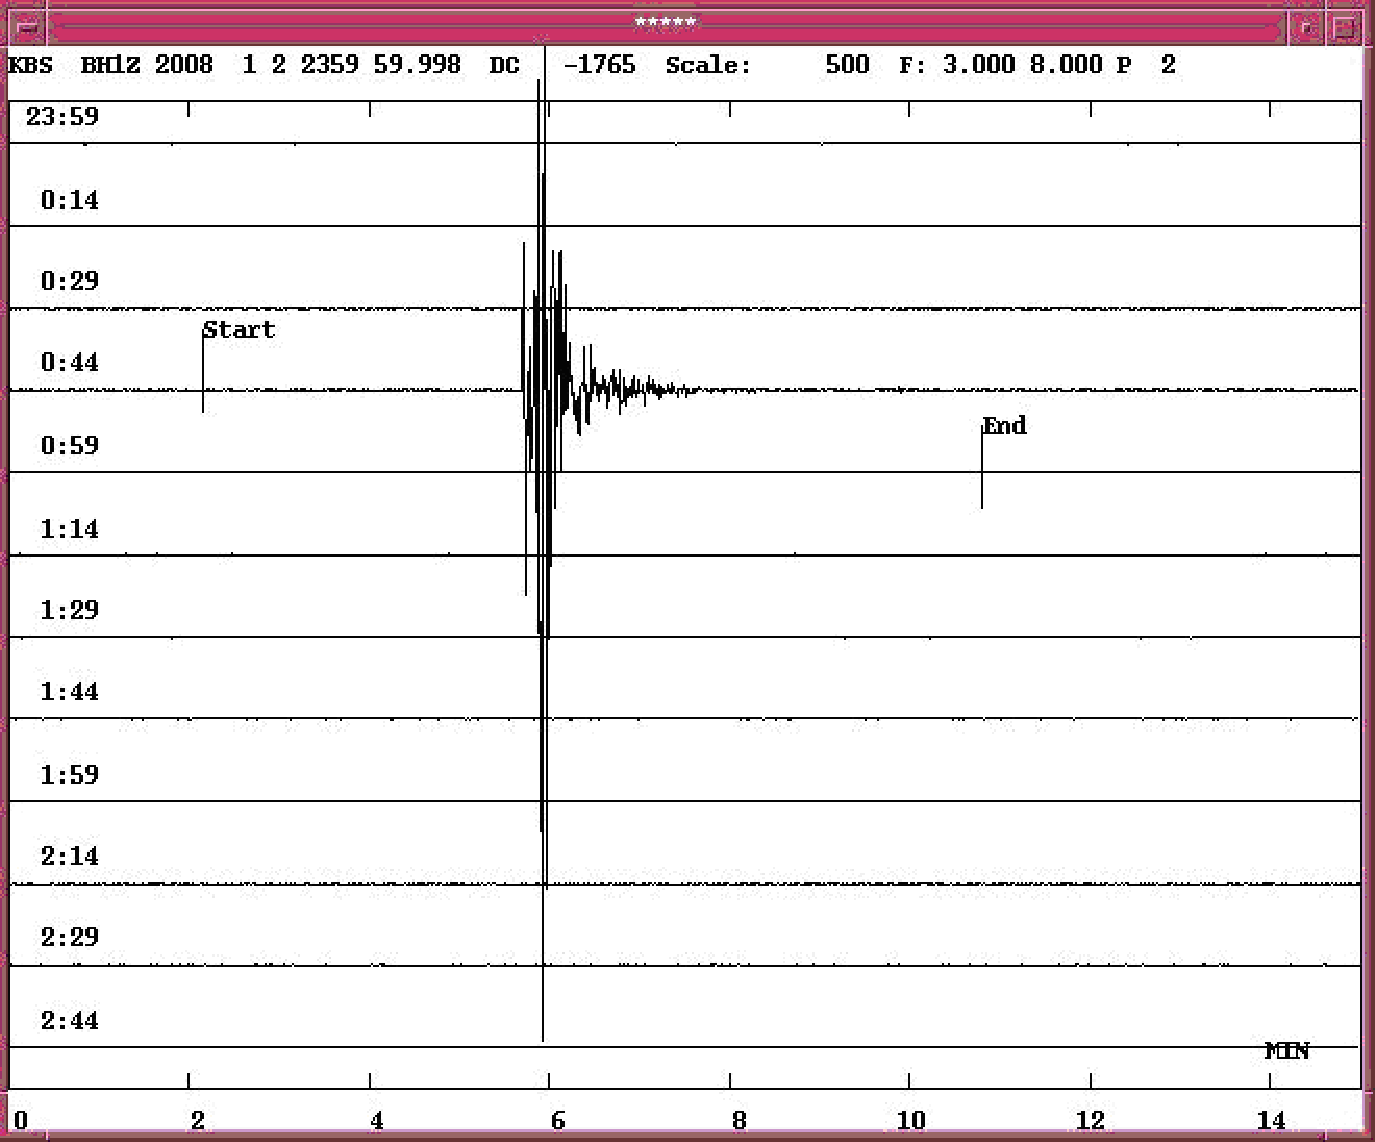
\includegraphics[width=0.9\linewidth]{fig/fig16}}
\caption{Example of time marks at the ``Start'' and ``End'' of an 
event recorded at the KBS station. The time marks is witten to the file 
\texttt{mulplt.ext} for data to be extracted and processed. Type ``s'' and ``e'' 
to add time marks.}
\label{fig:mulplt.ext}
\end{figure}

\subsection{Commands in MULPLT, overview}
\label{subs:commands-mulplt}

When the trace(s) are on the screen and the cursor is displayed, then several options are available. Most options can be displayed by pressing the MENU button in the upper right hand corner. Pressing MENU again removes the option boxes. Commands can be given by either pressing a letter or clicking on a box in the menu (Figure 
\ref{fig:mulplt-menu}
). By pressing ? or clicking on the Help button, the following help menu will be displayed: 

Help on MULPLT 

%\verbatiminput{include/mulplt.help}
\verbatiminput{include/MULPLT.HLP}

\index{Zoom in MULPLT}\index{Channel selection} \index{Filters in MULPLT}
\textbf{Filters in MULPLT}



All filters in MULPLT are Butterworth filters in time domain. When a filter is selected. using a hotkey or from the menu, the filter is only run one way, forward in time, and the number of poles is then 4. This will make a small phase delay where the first onset might appear a bit later, so if possible, read on unfiltered traces. If a 2 way filter is desired, press the filter key twice and the\index{Picking phases, use of filters} filter will also run backwards in time and the filter will be similar to an 8 poles filter. This gives theoretically a zero phase shift filter, however in practice, some of the onset energy is seen well before the first arrival, so it seems to distort the arrival times much more than using the 4 pole filter. When the program asks for a non fixed filter like when using the "." (Filt) command, the filter is always 4 poles by default. However, it is now also possible to interactively select number of poles and number of passes (1: forwards, 2: both ways)  using the ' command. Press ' and the user is asked for filter frequencies, number of poles (<10, but more then 4 and the filter might become unstable for high sample rates) and number of passes. In addition LP (low pass), HP (high pass) and BR (band reject) filters can be used. E.g for a 5-10 Hz filter some of the choices are:

\begin{verbatim}
5 10        4 pole band pass, command .
0 10        4 pole low pass, command .
10 0        4 pole high pass, command .
-5 10       4 pole band reject, command .
5 10 2      2 pole band pass, command '
\end{verbatim}
\index{Low pass filter}
\index{High pass filter}
\index{band reject filter}
\index{Filter, number of poles}
\index{Number of poles, filter}

WHEN PLOTTING, THE FILTER LIMITS, NUMBER OF POLES AND NUMBER OF PASSES IS WRITTEN ON THE SCREEN.

For band pass filters, the number of poles for both frequencies is the same. When doing spectral analysis or response removal and specifying a filter before, the filtering is done in time domain and the filter has the number of poles specified by the user, default 4. NOTE:\index{Filter and spectral analysis}When reading\index{Polarity} polarities, DO NOT USE FILTER, if possible.

Filtering and instrument correction: Since filtering is done in time domain, there is an added stability filter in frequency domain to avoid low frequency blow up. This filter is a 4 pole HP filter at 1/5 the filter low frequency corner. \index{instrument correction}

Filter limitations: For frequencies below 0.5 Hz, only 4 pole BP and BR filters can be used. If the user try to select another number of poles, the number of poles is set to 4.  

Filtered output: Extracting data with WAVETOOL, option 'Out'. It is only possible to use 4 pole BP filters, forward in time, using any other filter and the data is not filtered. Using option OutW  any filter can be used.


Prior to version 9.1
MULPLT used a 4 pole Butterworth filter in time domain and an 8 pole Butterworth filter in frequency domain. The filters in frequency domain were use in connection with instrument response correction and spectral analysis. It has turned out that the frequency domain filters distorted the signal in some cases, particularly for narrow band and low frequencies. Therefore, frequency domain filters are no longer generally used.  The change in filter setup, might change Ml magnitudes by 0.05 to 0.1 depending on which filter (if any) was used.

\begin{comment}
taken out 2012-01-27:
\textcolor{red}{pv-change: 
MULPLT uses a 4 pole Butterworth filter that can be used forward and backwards. Normally when a filter character or filter menu press is selected, the filter is only run one way and the number of poles is then 4. This will make a small phase delay where the first onset might appear a bit later, so if possible, read on unfiltered traces. If an 8-pole filter is desired, press the filter key twice and the\index{Picking phases, use of filters} filter will also run backwards. This gives theoretically a zero phase shift filter, however in practice, some of the onset energy is seen well before the first arrival, so it seems to distort the arrival times much more than using the 4 pole filter. When the program asks for a non fixed filter like when using the `.'(Filt) command, the filter is always 4 poles. When doing spectral analysis and specifying a filter before the spectral analysis, the filtering is done in frequency domain and the filter is 8 pole Butterworth. \index{Filter and spectral analysis}When reading\index{Polarity} polarities, DO NOT USE FILTER, if possible. If a filter is chosen from the menu, it is always 4 pole. 
\newline
The filter pass-band limits can be changed in \texttt{MULPLT.DEF}.\index{Change filters}. The user can also chose between two filter routines: bndpas (default) and recfil. 
\newline
The filter used in continuous mode can be either bandpass, low pass or high pass. Specifying a filter limit of zero, means that the filter is low pass or high pass. Limits of 0 10 Hz means a 10 Hz low pass filter.\index{Low pass filter}\index{High pass filter} 
}
\end{comment}

\textbf{Displaying uncertain time}

In each trace header in the SEISAN waveform file, there is a flag to indicate if the time might be uncertain (see Appendix \ref{app:seisan-format}). If that flag has been set, the message `UNCERTAIN TIME' will be displayed on top of the trace. Currently this flag is only put into the waveform files if the data comes from a SEISLOG system that has detected a timing error\index{Uncertain time}\index{Timing error} or if the data is converted from SEED/MiniSEED data. Simlarly plotting SEED/MiniSeed data, uncertain time will be displayed if that flag is set in any block in the time window read in for a particular trace. 

\begin{figure}
\htmlimage{scale=2.0}
\centerline{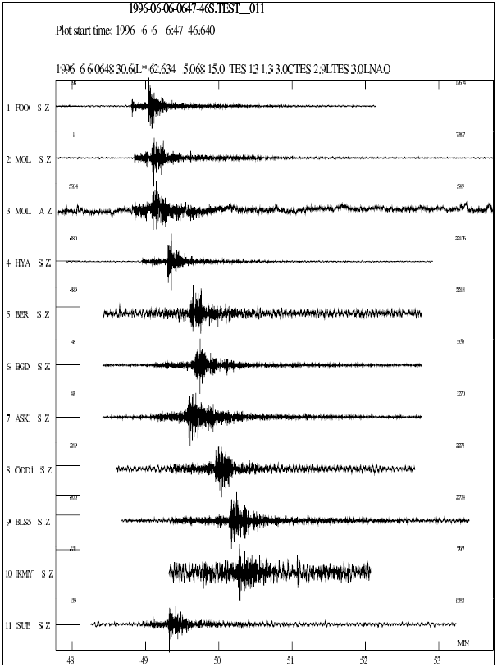
\includegraphics[width=0.9\linewidth]{fig/fig17}}
\caption{
An example of using MULPLT in multitrace plot mode. Notice that start and stop times are different for different channels. The horizontal line at the start of the plot is the \index{DC level}DC level. The small number above each trace to the right is the max absolute count with the DC-level subtracted and the small number to the left above the trace is the DC level. If plotting from EEV, the phase picks available are shown. 
}
\label{fig:mulplt-multitrace}
\end{figure}

\begin{figure}
\htmlimage{scale=2.0}
\centerline{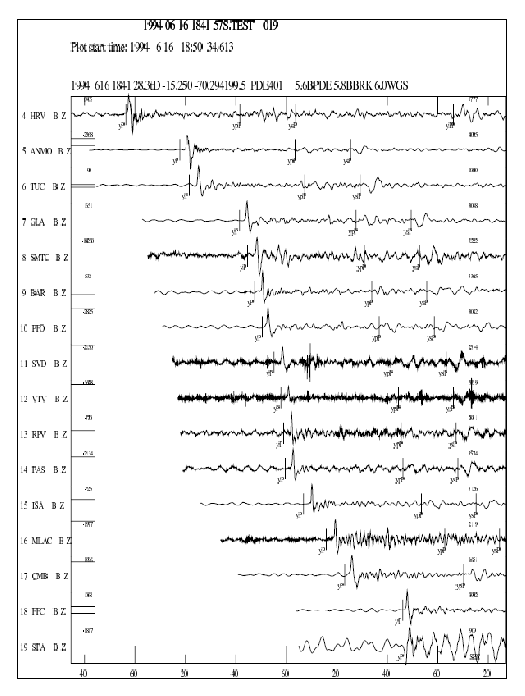
\includegraphics[width=0.9\linewidth]{fig/fig18}}
\caption{Examples of MULPLT with theoretical arrival times of some global phases. Short period seismograms are shown. The theoretical phases are marked with onset y below the trace and the read phases are marked normally above the trace. 
}
%\label{fig:mulplt-iasp}
\end{figure}

\begin{figure}
\htmlimage{scale=2.0}
\centerline{\includegraphics[width=0.9\linewidth]{fig2/fig2c}}
\caption{Example of MULPLT with theoretical arrival times showing global phases on a long period seismogram. The filter used from 0.01 to 0.1 Hz. Without filtering, almost nothing would have been seen on this broadband station. 
}
\label{fig:mulplt-iasp}
\end{figure}

\begin{figure}
\htmlimage{scale=2.0}
\centerline{\includegraphics[width=0.9\linewidth]{fig2/fig2d}}
\caption{MULPLT in continous mode.\newline
The plot shows 6 hours of long period data. The scale is 3000 counts 
between the traces and the filter used is from 0.01 to 0.1 Hz. The 
trace start time in hours and minutes is given on top of each trace. 
On the header line, P1 means the first page and DC is the DC level 
subtracted. Note that the numbers on the time scale at the bottom 
only are valid for the first trace unless all traces are 60 sec or 
60 min long.}
\label{fig:mulplt-cont}
\end{figure}

\begin{figure}
\htmlimage{scale=2.0}
\centerline{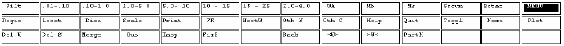
\includegraphics[width=0.9\linewidth]{fig/fig21}}
\caption{Example of the menu, which can be displayed on top of the plot.
}
\label{fig:mulplt-menu}
\end{figure}

Below is some more detailed description of some of the options. The one letter command is given 
with the menu command in parenthesis: 

To apply filters, first make a selection of options (filter, window, channel selection) and then execute by pressing R(Plot) (or selecting a zoom window). Figure 
\ref{fig:mulplt-multitrace}
shows an example. 

\index{Phase picking mode}Single trace mode: \index{Single trace mode}

In this mode, one trace is initially displayed on top of the screen, see example on Figure 
\ref{fig:mulplt-pick}.
The traces used are the ones earlier selected and will be displayed one by one. Several options are now possible as can be seen on the menu. Normally no hardcopies are made in single trace mode\index{Hardcopy in single trace mode} since it is intended for fast routine work. However, by starting MULPLT in multitrace mode (option 2) and then go to single trace mode (command T(Toggl)), hard copy files are made. 

Multitrace mode: 

In this mode hard copies can be made. If option 2 is used, both screen plot and hard copy files are made. If replot is made, only the last plot is available in the hard copy file. If option 3 is used, which is only hardcopy, there will be additional questions about, window length, start time, scaling and filters. If the scaling is set so that the plot occupies more than one page, several pages will be printed. If in this mode, \texttt{filenr.lis} is given as file name, the program assumes that all the files should be plotted and the only questions will be about the scaling and filters. All channels in each file will be plotted. This option is useful for plotting a large number of events with a single command. 

All channel mode\newline
In this mode, all channels for selected stations are displayed in a new window. This mode is particularly useful for working with three component data. By selecting one or several stations in multrace mode, all components for those stations will be displayed in new window by pressing y or ALLC on menu. Similarly in single trace mode, prsssing y or ALLC will display all channels for that station. The user can then go back to e.g. multitrace window and select another station to work with in three component mode.
\index{All channel mode} \index{Three component plotting}

Multiple screens in multitrace mode 

If many channels are available (like more than 30), it might be difficult to distinguish all and the channels can be displayed in multiple screens. The number of channels per screen is set in \texttt{MULPLT.DEF}. The number of windows or screens for a particular data set is given in top left hand corner as e.g. `Win 2 of 7' meaning current window is number 2 of 7 windows. To move to the next window, use TAB or NextW in menu. In each window, normal operation can be done. Channels selected will be kept. Using a large data set, the user can then view each window separately, select the channels of interest and when all channels have been viewed, only the selected channels will remain for display.
It is possible to togle between showing all channels and multiple screens by pressing N.  


Plotting stations in a given distance range
\index{MULPLT, plotting station in a max distance}
\index{Distance range, plotting}
When many stations are available, it might be useful to only plot only the stations nearest the epicenter or a particular location. For this option to work, parameter MULPLT AREA in  MULPLT.DEF must be set to a value larger than 0.0.  Then only channels with a distance ( radius degrees) larger than a given value from a point (midpoint) will be selected for plotting. The options for MULPLT AREA are:

1: midpoint from epicenter in S-file, radius from MULPLT.DEF
2: --------------------, ---------------------------- interactive
3: midpoint and radius from MULPLT.DEF
4: midpoint from MULPLT.DEF, radius interactive
5: midpoint and radius interactive

If interactive options are selected, the question(s) will come out just before plotting. Once a plot is made, the radius can also be changed interactively by using command R in multitrace mode. After selecting a new radius, the channel selection screen will come up with the channels selected. This option is not dependent on stations already being present in the S-file since all station information is taken from the STATIONx.HYP file.



\index{Channel order}Channel order in multitrace mode: 

Normally channels are plotted in alphabetical order according to station name, see parameter CHANNEL SORTING in \texttt{MULPLT.DEF}. They can also be plotted in the order they are stored in the waveform file(s) (option NSORT\_DISTANCE set in \texttt{MULPLT.DEF}). By setting the channel order parameter in the \index{MULPLT.DEF}\texttt{MULPLT.DEF} file, it is also possible to plot the channels in distance or time order. If MULPLT is started from EEV (and distance ordering is set), the channels will be plotted 
%\textcolor{red}{jh-change: 
in distance order provided distances are given in file. 
\index{Distance order}. 
Since there is no consideration for channels for the same station, the channels for one station, will be plotted in the same order as given in the waveform file. If a station is not found in the S-file, it will be plotted last. If plotting is done with MULPLT directly with a waveform file, the plotting order will be the start times as given in the waveform file header. Channel ordering can be turned on with the key "-" or pressing (Dist). If set in the \texttt{MULPLT.DEF} file, it 
is set when MULPLT starts up. It cannot be turned off for a given event when set from MULPLT but the flag is returned to the default value for the next event. 

Plotting from continuous data base 
\index{Continuous data}\index{Plotting continuous data} 

If a continuous data base is set up (see section \ref{subs:cont-data}), it is then possible to plot all traces from the continuous data base with MULPLT. \index{Cont}\index{Mulplt, option cont}When MULPLT starts up, use option cont and the user is prompted for a start time and interval. MULPLT will now check all continuous data bases for available data in required interval and display the available data. The forward (next) or back option will display previous or next window respectively. There is an 25 \% overlap between windows. If no data is available for the whole window, no trace is shown. If the beginning and the end is available, a line will join the two segments. If only end or beginning is available, only the available data is shown. All normal operation can be done on the window plotted so it is possible to e.g. extract data. If the register option is used, the whole window is extracted from the continuous data base as one file, copied to WAV and the S-file created. 

\subsection{Registering new events into SEISAN}
\index{New events into SEISAN}

Mulplt is the main tool for checking and putting new events into SEISAN. New events with waveform data can appear in two ways in SEISAN: 

\begin{enumerate}
\item
 Unprocessed waveform files are available in a work directory and have to be inspected and possibly put into the database. No S-files have been made. 
\item
 Raw data has already been put into a SEISAN database with S-files and corresponding waveform files in some work directory, the data has not been checked. This process has most likely been done with the automatic data collection software SEISNET \citep{ottemoller1999}, however, events can also have been auto registered with program AUTOREG.
\item 

Registering from continuous data: SEISAN continuous data base, BUS or SeisComp archives or a large SEED file.

\end{enumerate}

In both cases above, the aim is to inspect an event and decide if the event is real and should be put into the database using option `p'. All work must be done from the directory where the raw waveform files are located. The process of putting an event into the database results in creating the S-file (option1), giving the event identifiers and copying the waveform files of registered events to the waveform directory.By pushing p(Regis), the user will be prompted for \index{Distance indicator}distance indicator, which has to be L, R or D for local, regional or distant event. It is possible here to enter 2 characters like LE or LV for local explosion or local volcanic event. The \index{Event type}event type or \index{Event ID}event ID can be any character. Four characters are predefined and should only be used if the following definition correspond: P(probable explos\index{Explosion}\index{Volcanic event}ion), E(explosion), Q(confirmed earthquake) or V(Volcanic event). If the user enter L, R or D in lower case, the case will automatically be changed to upper case. The same also happends with E, P, Q and V. A third cahracter can optionally be entered for the model indcator \index{Model indicator}  which is put into column 21 of the header line. The volcanic events have a sub classification which can be entered when registering an event as volcanic, see section \ref{sect:volcanic}. The process of registering the event into the database implies that a new S-file is created or registered and in the S-file. An operator ID will be asked and the operator ID will be put on the \index{ID-line}ID-line. The question about operator will only be asked for the first event since it is assumed that all subsequent events are put into the same database by the same operator. The event ID, can later be used with the SELECT program to select out particular event types. When first putting an event into the database, the user is also prompted for database.  

Option (1) \newline
Data is available as waveform files only and a list of files must be 
made first with DIRF. Main option 0, 1 or 2 can be used for plotting. 
The `p' option creates the S-file and copies the waveform file to 
the WAV directory. The waveform file remains in the working directory. 
Unwanted waveform files can also be deleted so that when all events 
have been put in, only waveform files of `real' events remain in working 
directory. These can then be plotted with one run of MULPLT, see 
section \ref{subs:mulplt-main}.  

Option (2) \newline
Data is available already in a database, however since the data has not been inspected, the waveform files are still in a work directory. In EEV, the first unprocessed event in the month is found 
with command `ss' and MULPLT is started with command `po' to invoke all defaults. If the event is to remain in the database, it must be registered with option `p'. The process and the questions are the same as in option (1) except that the S-file is not created since it is already there. The S-file is cleaned for all processing information from SEISNET\index{SEISNET}\index{Delete S-file}\index{Delete waveform file} if present. This normally also includes automatic phase picks. However, they can be kept if parameter REG\_KEEP\_AUTO is set in the \texttt{SEISAN.DEF} file. \index{REG\_KEEP\_AUTO}\index{Delete automatic picks}The status of the files also changes to being newly registered as under option (1) (see definition of processing codes in Appendix 1) and waveform file(s) copied to WAV. Before registering, it might be an advantage to merge waveform files and delete unwanted files (could be false triggers), see section \ref{subs:commands-mulplt}. Files can only be merged and deleted in working directory with commands Delw and Merge (Menu). In this process of putting new events into the database, it is also an advantage to delete unwanted events. This is done with option `S'(Del S)'. The S-file is deleted, but the waveform files remain in the working directory. 

Option (3) \newline

When reading continuous data, an output file can be made with the Out option and that output file can be registered. However, it is also possible to do this in a single operation using the Register option like above. The selected time window is then extracted, the waveform file copied to WAV and the S-file registration made. In addition to the questions above, one additional question is given: 

Output channels on screen (s) or all channels(enter)

This option is intended to be used with routine operation when many channels are present and the user only views a few, like all vertical channels, but want to extract (and register a file with all channels).

\index{Preprocessing of data}Preprocessing of data while registering new events, option (1) 

Normally a series of events are registered first and MULPLT terminated. Then EEV is started up for interactive picking and location. However, if preliminary processing is desired while registering the event, this is also possible. 

\index{Registration and preprocessing}Phase picks:If phases are picked before the event is registered, these readings are saved in the database at the time of registration. After the event has been registered, MULPLT automatically goes to the next event in FILENR.LIS and no more phase picking can be done. 

Processing with a given program: 
Optionally MULPLT can, after registration, start any program processing the newly registered event. 
E.g. the AUTOPIC program can be started or a program reading amplitudes etc. The program name is defined in \texttt{MULPLT.DEF}. 

Locating the event: As the final step after registration, the event 
can optionally be located and the location optionally placed in the 
database. \newline
The above options have been put in on the suggestion of Brian Baptie, who is using it for rapid processing of volcanic events, where in most cases the operator only wants to look at the event once. 

\subsection{Adding BUD archive waveform data to nordic file, WAV2BUD}
\index{Adding BUD archive to nordic file}
\label{page:wav2bud}


The program WAV2BUD reads nordic files like \texttt{collect.out} or 
\texttt{select.out} and add lines (type 6) to each event in the input file 
that link to the waveform data in a BUD archive.
Note, it is only the data given in \texttt{SEISAN.DEF} by the 
ARC\_CHAN parameter that are linked to. The events with the 
new data link is listed in the \texttt{budfile.out} file.\newline
The program is written by \textbf{Ruben Soares Lu\'is}.

\subsection{Phase picking, amplitude, weight and polarity}
\index{Phase picking}

Picking phases: 

The plot will display any pick present in the database (current S-file). To pick new phases, position cursor at phase, and press the key as indicated on top of the screen (if in Single mode). E.g. pressing 1 will read IP. Pressing the same key again with the cursor at a different place will delete the old one (indicated with a D) and display the new one. Additional default phases, which can be picked, are i for I, e for E and A for AMP (note upper or lower case). Keys for phases have default definitions, but can be redefined using the file \texttt{MULPLT.DEF}, see below. The end of the coda is picked as a phase (C) and the program calculates \index{Coda length}coda length IF AND ONLY IF A P-READING IS PRESENT. 

Picking amplitudes: 

Position the cursor at the bottom or top of a wave and press a, then at the other extreme (bottom or top) and press a (do not use upper case, see below). There is no requirement for going left to right or top to bottom, it can be done in any order as long as the two extremes are marked. At each press, a cross is marking where the pick was made. In case a filter, like WA, MS or Mb is applied, the program will associate the amplitude with the respective amplitude reading (AML, AMS or Amb). \index{Phase AMP}\index{AMP} Amplitude and period are calculated and stored with the phase. Otherwise, if none of these filters are applied, a menu pops up and the user needs to select a phase name to which the amplitude and period readings are associated. It is often a good idea to store amplitudes with the nondescript phase E, I or AMP since it then will remain even if the phase is deleted or changed. If an attempt is made to pick amplitude on a trace which is not in nm, the reading must be confirmed since SEISAN assumes all amplitudes to be in nm (see section on instrument correction). If no phase is picked, no amplitude is stored. The amplitudes are always assumed to come in pairs so if 
e.g. 3 amplitude values have been picked, and the user tries to pick a phase or quit the program, it will appear frozen since the program is still waiting for the next amplitude measurement. It is always the last pair of amplitude measurements, which are used. Amplitudes can be picked on both corrected and uncorrected traces.\index{Problem, picking amplitude} 

If A is pressed instead of a, the amplitude is read and marked automatically. It works in most cases, but sometimes two subsequent peaks are not correctly chosen and the amplitude reading has to be done manually. The method is to find the absolute extreme and then the largest amplitude before or after is selected in order to obtain the peak to peak amplitude, from which the amplitude is calculated by dividing by 2. For more information, see.  ../LIB/auto\_amp.for.\index{Amplitude, automatic}\index{Automatic amplitude} 

\index{Component names in S-file}Component names when picking phases: 

In the S-file, the component only has 2 letters while in the waveform file it has 4 letters. There must therefore be a unique translation between the two. This definition is given in the subroutine componen.for\index{Componen.for} in LIB. Most common combinations are now defined, however if a new one is defined in the waveform file which does not exist in componen.for, the first and last letter of the input component will be used. If e.g. an input component is called SS Z, then the code in the S-file will be SZ. This means that picks for stations with components, which do not differ in first and last character, cannot be separated in the S-file. Component names for rotated channels will be e.g. SR and ST for short period radial and transverse components respectively. 

Reading \index{Polarity}polarity: 

If the cursor is above or below the trace at a distance marked by horizontal tics on the sides of the plot, the first motion is also picked and displayed. Do not use a filter if possible.  
Assigning w\index{Weight}eight: 

A phase can be assigned a weight. Move the cursor close to a pick and press one of the keys 1-9 in \index{UPPER case}UPPER case thus using e.g. !"\# (default, can also be changed), and a \index{HYPO style weight}HYPO style weight is assigned and displayed. Although weights 0 to 9 can be put in, HYP only uses 0-4 and 9 (see section \ref{subs:hypocenter-program}). Phases with associated \index{Amplitude}amplitude, \index{Period}period, \index{Azimuth}azimuth or \index{Apparent velocity}apparent velocity are displayed with a hat below on the phase indicator line. The default keys for the weights might not be correct on all keyboards, if not, set keys in \texttt{MULPLT.DEF}.  

Automatic determination of coda length\index{Automatic coda length}\index{Coda length} (C or c): 

The coda length can be quite variable among different operators and a function has been made to automatically determine the coda length. The signal is bandpass filtered and the end of the coda is determined by a standard STA/LTA procedure. The parameters are set in the \texttt{MULPLT.DEF} file. Press C to find coda length automatically or c to determine manually. If parameter CODA AUTO is set in \texttt{MULPLT.DEF}, c I sused. The coda length can only be determined if a P-phase is present. 

\subsection{Theoretical arrival times for global and local phases and location}
\index{Global phases} 

In order to assist in \index{Identifying seismic phases}identifying seismic phases, there is an option for displaying the theoretical arrival times of several global and regional phases while picking phases. The steps to do so are the following: 


\begin{itemize}
\item[1]
 Before entering MULPLT from EEV, the theoretical travel times have to be calculated for the current event. This assumes that the origin time and hypocenter is given in the header line or a subsequent type one line. If not, enter manually (from e.g. PDE) or use the EEV command INP\index{INPUTEPI}UTEPI or IN\index{INPUTONE.}PUTONE. Then proceed to calculate the theoretical arrival times using EEV command IASP with the \index{IASPEI91}IASPEI91 traveltime tables (for more details, see section \ref{subs:iasp}). The same command is also available inside MULPLT in multitrace mode. All arrival times (or a subset, see \ref{subs:iasp}) for all stations in current S-file will now be calculated with program IASP and stored in file iasp.out (no importance for the use, just for information). See Figure 
\label{fig:mulplt-multitrace}
for an example in multitrace mode. Note that very many theoretical phases can be generated if the S-file has many stations. MULPLT will stop if more phases are used than the di\index{Dimension}mensions are set up for (include file seidim.inc), and you must use fewer phases (a warning is given when 500 phases are generated) or set up SEISAN with larger dimensions, see section 3. Theoretical local crustal phases for the current model can  be calculated with program WKBJ and displayed, see section \ref{sect:synt-seismogram}. Theoretical phases can also be calculated when using the location option, see next section. 

\item[2]
 Pick phases: When a trace is displayed on the screen, all theoretical phases inside the time window will also be shown. To distinguish the \index{Theoretical phases}theoretical phases, they are prefixed with a y and displayed below the trace (normal phases have I, E or blank and are displayed above the trace). Position cursor where you see a phase which you think corresponds to a theoretical phase and press y. The nearest theoretical phase will now be placed at that position with a prefix E. Only theoretical phases selected in this way will be written in the S-file. Note that the phase names can be up to 8 characters long, see Appendix 1 for the definition of \index{Long phase names}long \index{Phase name}phase names. 
\end{itemize}

If the phases fit badly, start looking at the P-phase. If that does not fit the theoretical P-phase, change the origin time in the S-file so that the P-arrival fits, and recalculate the theoretical phases.  

PROBLEM: In multitrace mode, only one theoretical phase can be picked. Replot must be made before picking the next. \index{Problem, reading synthetic phase}

Locate earthquake \index{Locate event in MULPLT}

If several phases have been read and saved in the S-file, the event can, in multitrace mode, be located with command l (Locat), just as in EEV. The screen is cleared and the usual location rolls over the screen. When the location is finished, the plot will reappear and the calculated travel times will be displayed as synthetic phases (see previous section). In this way it is possible to immediately visualize the differences between the read and calculated phases. The output files are \texttt{hyp.out} and \texttt{print.out} as usual. 

\subsection{Instrument correction and magnitudes Ml, mb and Ms}
\index{Ground motion seismogram}

The correction for instrument response is done by taking the spectrum of the selected window of the trace, dividing with the response function and converting back to the time domain. Any filtering specified is done in the frequency domain. Filtering is needed in most cases. 

Ground motion 

Option g(Groun) removes the effect of the instrument and displays a ground motion seismogram. After selecting g and the zoom window, there is a question of which type of seismogram to calculate: \index{Displacement}Displacement (d), V\index{Velocity}elocity (v) or \index{Acceleration}Acceleration (a). The corrected trace is shown below in \index{Nanometer}nanometers(nm), nm/sec or nm/(sec*sec) (if \index{Response file}response information is available). Note that this might produce strange seismograms, since e.g. a SP seismograph has very low gain at low frequencies so noise might be amplified very strongly. It is therefore recommended to also do some filtering when using the g option. 

Amplitude for determining Ml 

For the w(WA)-option \index{Wood Anderson}(Wood Anderson), the trace is corrected for the instrument to produce displacement. The displacement trace is then multiplied with the response of the Wood-Anderson instrument to produce a signal to look exactly like it would have been seen on a Wood-Anderson seismograph. The maximum amplitude (nm) is read and saved to the S-file with name IAML. The Wood-Anderson response (PAZ) is hardwired in SEISAN and it is similar to a 2 pole Butterworth high-pass filter at 3 Hz.   In SEISAN versions prior to 8.3, a fixed 8 pole bandpass filter was used (1.25 Hz - 20 Hz). Filtering is done in the frequency domain. For noisy traces it might also be required to put a filter at the high end. This can be specified in the \texttt{MULPLT.DEF} file. Unfortunately, the correct low cut filter with 2 poles will often result in the seismogram blowing up at low frequencies and might be quite useless for earthquakes with magnitude below 2.0 - 2.5  So in addition to the PAZ filter, a fixed bandpass filter can be added (see \texttt{MULPLT.DEF}). In the standard distribution of SEISAN, this additional filter is set to an 8 pole filter at  1.25 - 20 Hz. In all cases where an additional filter is used, the read amplitude is corrected for the filter gain and the true ground motion written in the S-file will be larger than the amplitude seen on the screen. The additional default filter probably only makes a difference for very large events (Ml $>$ 5). Other filters at a higher frequency should only be used for small events (M$<$1) .  NOTE: In SEISAN version 7.1.1 and earlier, the low cut filter was set by mistake to 0.8 Hz. Repicking amplitudes with the correct filter might change magnitudes of larger events slightly.

Displaying response information 

The response function for the current channel can be shown with option `:' (Resp), see Figure 
\ref{fig:mulplt-resp}.
If no response function is given, a message is shown. If the response function is taken from the waveform file header instead of from the CAL directory, a message is given. \index{Response, from where}\index{Response, show curves} 


Amplitude for determining \index{mb}mb: 

Determining mb assumes that the maximum amplitudes are measured on classical 1 Hz WWSSN instruments having a peak gain around 1.5 Hz. This in reality means a band limited measurement.  To pick ground amplitudes for determining Mb on instruments with a broader or more narrow frequency band, like most high frequency SP instruments, some filtering must first be done. Using the j(mb)-option, the trace is corrected for the instrument to produce displacement. The displacement trace is then multiplied with the response of the SP WWSSN instrument to produce a signal to look exactly like it would have been seen on a SP WWSSN seismograph. The unit of the amplitudes seen on the screen is nm, however the amplitude will only represent the ground motion correctly at the frequency of the maximum gain at 1.5 Hz and for all other frequencies, the true ground motion will be larger than seen on the screen. The maximum amplitude is now picked and displayed below the trace, corrected for the gain relative to the gain at 1.5 Hz and written to the S-file with name IAmb. This means that the amplitude written to the S-file generally will be larger than the amplitude displayed on the plot. The SP WWSSN response (PAZ) is hardwired in SEISAN and cannot be modified with filters.

In SEISAN version to 8.2.1, the default filters used to simulate SP WWSSN were, by mistake, in the band 0.9 (2 pole) to 1.8 Hz (3 poles). This will result in slightly wrong magnitudes unless the user had put in correct new filter contants... Prior to SEISAN version 8.2, the default filters used were 0.5 Hz (8 pole)  and  5.0 Hz (8 pole filter), which was close to the correct values. No correction for relative gain was used in SEISAN versions prior to 8.3.. All of these changes could have resulted in smaller errors in mb, which only can be corrected by repicking the amplitudes.

Amplitude for determining mB

Amplitude for mB is defined as the maximum velocity on a wide band instrument (0.2 -30 sec or 0.033 - 5 Hz). The maximum amplitude Vmax is measured on a velocity trace. Using the J(mB) option, a velocity trace (nm/s) in the frequency band 0.033 - 5 Hz is displayed. The maximum amplitude in nm/s (irrespective of frequency) is picked and displayed below the trace. This amplitude is now written to the S-file with phase name IVmB\_BB. In principle, mB can be calculated using any instrument, but in practice it can only be used if the P-signal is seen clearly on an unfiltered broad band velocity record.
The Butterworth filter 0.033 - 5 Hz , 8 poles, is hardwired and it cannot be modified with additional filters.

Amplitude for determining \index{Ms}Ms: 

The attenuation function for determining Ms assumes that the amplitudes are measured on classical LP WWSSN instruments having a peak gain around 15 second. To pick ground amplitudes for determining Ms on instruments with a broader or more narrow frequency band, like most broad band instruments, some filtering must first be done. Using the k(Ms)-option, the trace is corrected for the instrument to produce displacement. The displacement trace is then multiplied with the response of the LP WWSSN instrument to produce a signal to look exactly like it would have been seen on a LP WWSSN seismograph. The unit of the amplitudes seen on the screen is nm, however the amplitude will only represent the ground motion correctly at the frequency of the maximum gain at 15 seconds  and for all other periods, the true ground motion will be larger than seen on the screen. The maximum amplitude is now picked and displayed below the trace. This amplitude is then corrected for the gain relative to the gain at 15 seconds and written to the S-file with name IAMs\_20. This means that the amplitude written to the S-file generally will be larger than the amplitude displayed on the plot. The LP WWSSN response (PAZ) is hardwired in SEISAN and no additional filters can be used.

The attenuation function for determining Ms assumes that the amplitudes are measured in the period range 18 - 22 sec and it is up to the user to make sure that the the amplitude is in the correct range.. 

For SEISAN 8.2.1, the default filters used were in the band 0.038 (2 pole) to 0.1 Hz (1 pole). Prior to SEISAN 8.2 default filters were 0.042 to 0.063 Hz (8 pole filter). No correction for relative gain was used in SEISAN versions prior to 8.3. These changes might have resulted in small errors ins Ms and can only be corrected by repicking the amplitudes.

Amplitude for determining MS

Amplitude for MS is defined as the maximum velocity on a wide band instrument (3 -60 sec or 0.017 - 0.3 Hz). Using the K(MS) option, a velocity trace (nm/s) in the frequency band 0.017 - 0.3 Hz is displayed. The maximum amplitude in nm/s (irrespective of frequency) is picked and displayed below the trace and written to the S-file with phase name IVMs\_BB. In principle, MS can be calculated using any instrument, but in practice it can only be used if the surface wave is seen clearly on an unfiltered broad band velocity record. The big advantage with using MS is to avoid the 18-22 s limitation needed for Ms. The Butterworth filter 0.017 - 0.3 Hz , 8 poles, is hardwired and cannot be modified with additional filters.

Problem: If a long trace (large number of samples) is used, the instrument correction might fail (funny result seen) due to numerical overflow in the spectral conversion. Choose a shorter window. \index{Problem, instrument correction} 

\subsection{Determine azimuth of arrival (3 comp or array) and component rotation}

Azimuth of arrival from \index{3-component stations}3-component stations, h(Azim) 

If a 3 component station is available, the azimuth of arrival can 
be determined using the method developed by \citet{roberts1989}. 
Display any of the 3 components and press h (Azim). Then select a 
zoom window around the P-arrival of a few secs duration for the 
analysis. The 3 components will now be displayed below in order Z, 
N and E and the calculated azimuth, apparent velocity and correlation 
will be displayed at the bottom line. In order to check the stability 
of the estimate, try different windows and filters. Often, a filter 
must be used to get reliable results. The displayed azimuth and 
apparent velocity is only saved in the S-file when an associated 
phase is picked. THAT PHASE MUST BE PICKED ON THE SINGLE UPPER 
TRACE SEEN ON THE SAME SCREEN. If there is none, use I or E. The 
velocity estimate is not very reliable and is dependent on the local 
velocities. In order to calculate the apparent velocity, the P-velocity 
of the top layer must be given. The default value is 5.0 km/sec, but 
another value can be set in the \texttt{MULPLT.DEF} file. To get a 
good estimate, the correlation coefficient should be as high as possible 
and positive. The quality of the obtained azimuth can be tested by 
locating the event with the calculated azimuth weighted out and observe the azimuth residual. 
Figure \ref{fig:mulplt-3comp}
shows an example.

Azimuth and apparent velocity from array data, FK analysis\index{FK analysis}\index{Apparent velocity} f(FK) 

Using this command, the traces seen on the screen will be put into the FK program and an FK plot will be displayed. The azimuth and apparent velocity with the highest correlation is selected by the program, however any other value can be manually selected. The values will ONLY enter the S-file if associated with a phase in the same way as amplitudes are picked. For more details, see section \ref{sect:fk-analysis}.
% 6.29. 

\index{Rotated seismograms}Rotated seismograms 

Option u(Rotat) will rotate the \index{Horizontal component}horizontal components for the next plot if the two horizontal components are available. The rotation will display the radial component instead of the N-component and the transverse component instead of the E-component. The back-azimuth used is displayed above the trace. All channels will be displayed  rotated until u(Rotat) is pressed again This means that phases can be picked and spectra made with the rotated channel. When picking phases on rotated signals, these will appear in the S-file with components R or T instead of N and E respectively. This also means that only if the rotated signals are shown, will the phases read on rotated channels appear on the plot. The station b\index{Backazimuth}ack-azimuth is obtained in the following way: If a hypocenter is given in the header line, the angles are calculated using the current \texttt{STATIONx.HYP} file. If no hypocenter is available, the angle will be read from the S-file under column observed azimuth (47-51) (if not blank) and the azimuth residual will be added. This option permits the user to first determine the azimuth with the 3-component option and then rotate the signals with the determined azimuth. Finally, if no observed azimuth is available, the event to \index{Station azimuth}station azimuth + 180 deg. will be used if available (column 77-79). If no back-azimuth\index{Backazimuth} can be found, no rotation is done and an angle of 999 deg. is displayed. If in single trace mode and choosing the 3-component option AND the rotate option, the user will be prompted for a rotation angle and the rotated channels will be shown in the usual 3-component plot, however, the azimuth determined is done with the unrotated channels. 

\index{Problem, Rotation and removing response}PROBLEM: In general, the R-channel will use the response of the N-channel and the T-channel will use the response of the E-channel so for instrument response removal to be correct, the 2 channels must have the same response curve. 

\subsection{Data manipulation commands}

Select other channels: o(Oth) 

The channel selection menu comes up again. 

Go back one channel in single trace mode, go back one event in multitrace mode if MULPLT is started from EEV: B(Back) 

Select other waveform files from S-file: W(OthW) 

If more than one waveform file available for the event, one or several others  can be selected. 

Delete waveform files: 

This can only be done in multitrace mode: The command is d(DelW) and the cursor must be above the top frame of the plot. There are two possibilities: 
\begin{itemize}
\item[1]
Input is from \texttt{filenr.lis}: The current file is deleted and if in default mode, the plot moves on to the next event.\index{Waveform file, delete}\index{Delete waveform file} 

\item[2]
 MULPLT is started from EEV: If only one waveform file is available, the program proceeds as under (1). The waveform file is deleted and the waveform file entry in the S-file remains. However, if more than one waveform file is available, the user can use a menu to select which files to delete. Only the waveform file entries in the S-file are deleted, the waveform files remain. This option is mostly used with SEISNET. 
\end{itemize}

Delete S-files D(Del S) 

This command deletes the current S-file. It can only be used if MULPLT is called from EEV. No waveform files are deleted. 

Merge waveform files given in S-file M(Merge) 

The files will be merged\index{Merge waveform files}\index{Waveform files, merge} to one waveform file and the old individual file names removed from the S-file and replaced by the new file name of the merged file. The original waveform files remain. Files to be merged will be shown on a menu. Mostly used with SEISNET. The user MUST have files in working directory. If files are in the data base, they will not be shown on the merge menu. 

% jens
Overlay two channels: It is sometimes practical to be able to overlay 2 or more 
channels. The channels to be overlaid must follow each other on the screen (sorting might influence that). Move the cursor to the channel name of the lower of the two channels, press \& and the channel is marked with a cross. When doing replot, that channel will be plotted in red on top of channel above. Both channels will be autoscaled, but if absolute scaling is used, the real difference in amplitude is seen. Overlay cannot be deselected without leaving MULPLT. This option is particularly useful when comparing real and synthetic seismograms result form moment tensor inversion, see that section later. \index{Overlay channels in MULPLT}

Output of binary waveform file, O(Out) 

It is often useful to be able to select  part of a waveform file and save it. The Out option makes an output file of the traces AS DISPLAYED ON THE SCREEN with exactly the same channels, \index{Extract from waveform file}\index{Waveform file, extract from}and time window in a file with a standard SEISAN waveform name. The output format is alw\index{MERGE\_WAVEFORM}ays SEISAN, even if some input files have a different format. The network code in the file name will ALWAYS be the station code if all channels are from the same station  Otherwise the network code has the default name MERGE. Alternatively the parameter MERGE\_WAVEFORM can be set in \texttt{SEISAN.DEF}. The data is output exactly as displayed on the last screen, so if filtering or instrument response has been made, the output file will also be filtered or instrument corrected WITH SOME RESTRICTIONS: Not all response, channel or filter combinations are possible. Only 4 pole band pass filters can be used, no rotated channels and none of the magnitude simulated traces like Wood Anderson for Ml. if you want exactly what is seen on the screen for all combinations, use option \texttt{OutW}.  If any filtering or instrument response correction has been done, a note will be inserted in the SEISAN waveform header so the user can see that this is no longer the original data. The note could be e.g. ` Displacement 1.250- 20.0 Hz' indicating that output has been filtered and converted to displacement (nm). Note that numbers have been scaled so only if the SEISAN file is read with standard SEISAN routines, will the numbers be correct. If the output file is converted to ASCII by SEIASC, the number shown must be multiplied with a given scaling factor, see SEISAN binary format description (Appendix \ref{app:seisan-format}). There is no response information in the header other than the short text. Since the station code is still the same, it is technically possible to correct for the response again using the response information in the CAL directory, 
\textbf{however, be aware that this will give wrong results}.

Option \texttt{OutW}:This option will output the signal exactly as seen on the screen with all the selected filter and response combinations. It also handles rotated channels. The output file is \texttt{mulplt.wav} and it is an Ascci file with real numbers in Helmberger format (readable by SEISAN). To make the file, press \texttt{OutW} and wait for message '\texttt{mulplt.wav written}' in top right of the screen. For many channels and high sample rate it could take some time since the output is Ascii. If the traces in the window do not start and stop and stop at the ends, then dc levels will be added so all channels in the output file has same start and stop timers. Format description is found in section moment tensor inversion. \index{mulplt.wav} 

Output of ASCII waveform file 

This option only works if parameter SPECTRAL\_OUTPUT has been set in \texttt{MULPLT.DEF}. The output file signal.out contains the last data displayed in the single trace zoom window (in ASCII and real numbers). This option is a another way (see option O(Out) above) of getting an output file that has been filtered or instrument response corrected.  The main difference is that this file is only for one trace \index{Signal.out}\index{Extract data in MULPLT}\index{Output, corrected trace}written in ASCII. 

\index{Fixed scaling}Fixed scaling 

Normally all traces are plotted with au\index{Autoscaling}toscaling. However, it is sometimes useful to be able to scale the traces with a fixed scale in order to e.g. compare traces or override the autoscale in case a spike distorts the autoscaling. Option *(Scale) will prompt the user for a maximum count to use for the scaling of all traces. 

\begin{figure}
\htmlimage{scale=2.0}
\centerline{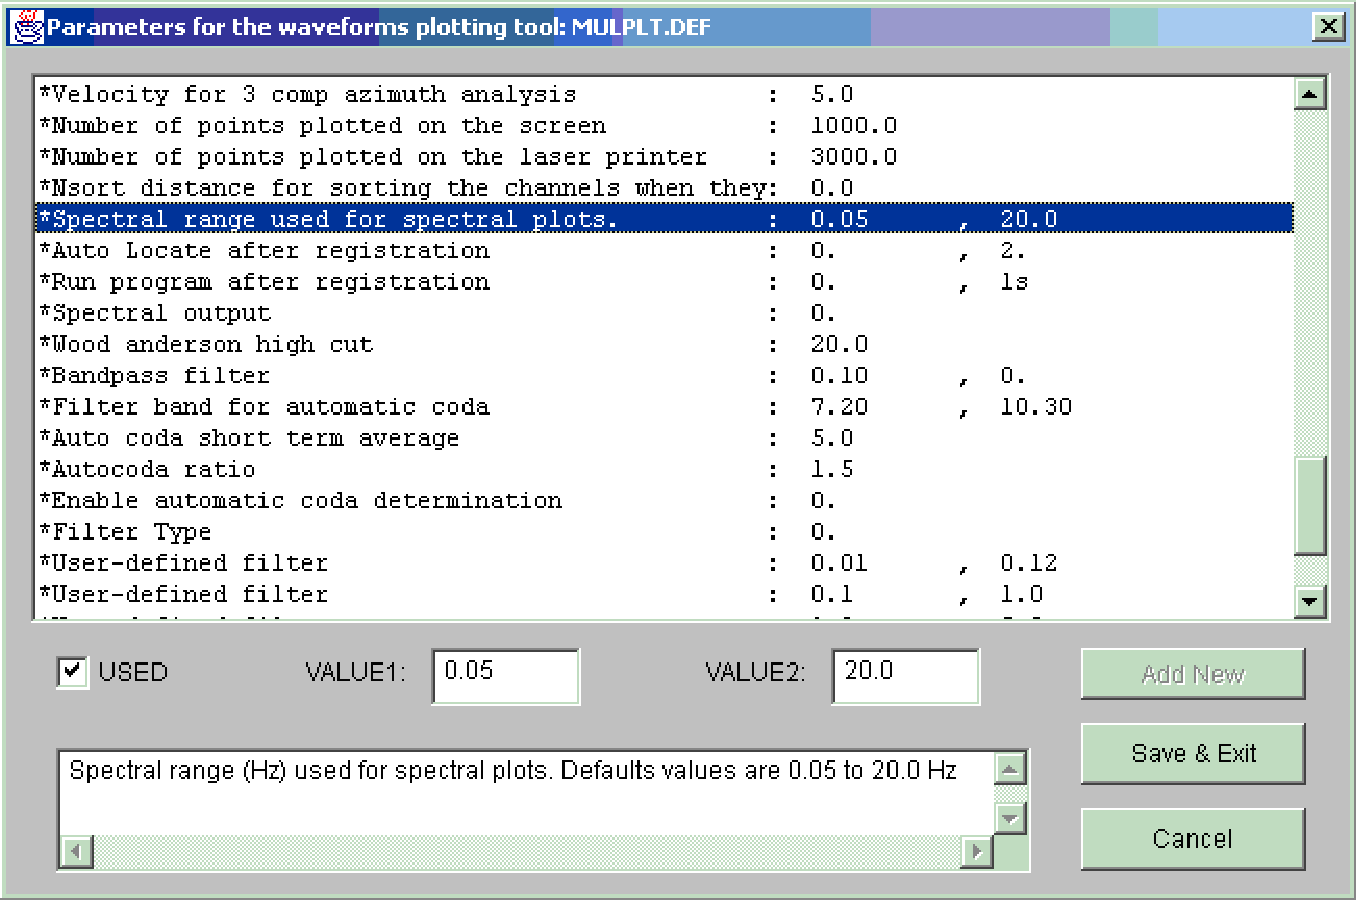
\includegraphics[width=0.9\linewidth]{fig2/fig3}}
\caption{Using MULPLT for picking phases. The top shows the original trace and the bottom the zoomed part. Note that the amplitude has been associated with the phase E and not the ESg. This means that if the S-phase is deleted, the amplitude will remain. 
}
\label{fig:mulplt-pick}
\end{figure}


Example of using MULPLT on SUN: 

Comments are given with ! in front 

This example shows how running MULPLT from EEV would look. 

\begin{boxedverbatim}
/top/seismo/REA/BER__/1991/01/01 0557 12L.S199101 ! S-file name
Read header from file /top/seismo/WAV/9101-01-0557-12.WNN_13

 Plot options:     Interactive picking          Return  ! first choice
                   Multi trace plot on screen, def (0) 
                   Multi trace plot on screen      (1) 
                   Multi trace plot on screen+laser(2) 
                   Multi trace plot on laser       (3) 
                   Multi trace plot on laser       (3) 
                   Continuous on screen            (4)
                   Continuous on screen + laser    (5)
                   Continuous on laser             (6)
                   Stop                            (9)
                       ! now comes a menu for selection and then
                       ! the plot appear in Single mode since a 
                       ! return was made
\end{boxedverbatim}

%\fbox{\verbatiminput{include/mulplt.eev.1}}
%\framebox{\verbatiminput{include/mulplt.eev.1}}
%\framebox{verbatiminput}

The next example shows how to plot many events in one go, first make a list with DIRF. 

\begin{boxedverbatim}
dirf 9101-10*                      ! events from January 10, 1991
#  1  9101-10-0915-15S.KMY_03  
#  2  9101-10-1510-55S.NSS_12  
#  3  9101-10-2333-44S.NNN_11  

mulplt
file name, number, filenr.lis for all   
filenr.lis             ! plot all events in filenr.lis
 Resolution in cm/sec, 0: plot all on one page (default)
0                      ! scale will be different for each plot!!! 
Read header from file:9101-10-0915-15S.KMY_03                   
 Page           1
 Channel:           1

Plotfile sent
Read header from file:9101-10-1510-55S.NSS_12       ! next event in list  
 Page           1
 Channel:           1
 Channel:           2
 Channel:           3
 Channel:           4
 Channel:           5
 Channel:           6
 Channel:           7
 Channel:           8
 Channel:           9
 Channel:          10
 Channel:          11
 Channel:          12
 
Read header from file:9101-10-2333-44S.NNN_11          
 Page           1
 Channel:           1

 ! etc.


Plotfile sent
Read header from file:9101-10-1510-55S.NSS_12       ! next event in list  
 Page           1
 Channel:           1
 Channel:           2
 Channel:           3
 Channel:           4
 Channel:           5
 Channel:           6
 Channel:           7
 Channel:           8
 Channel:           9
 Channel:          10
 Channel:          11
 Channel:          12
 
Read header from file:9101-10-2333-44S.NNN_11          
 Page           1
 Channel:           1

 ! etc.
\end{boxedverbatim}


\subsection{Spectral analysis, s(Spec)}
\label{subs:spec}

The spectral analysis option for local and teleseismic events is selected in single trace mode.  The spectral analysis is based on the \citet{brune1970} model and various assumptions about the geometrical spreading and anelastic attenuation. 

The theoretical \index{Source displacement spectrum}displacement spectrum d(f)\citep{brune1970} is: 

\begin{displaymath}
d(f) = G(r,h) * D(f) * Moment*KK /(1+f**2/f0**2)* (4 * pi * DE * V**3)) 
\end{displaymath}

where G(r,h) is \index{Geometrical spreading}\index{Source parameters}geometrical spreading, r is epicentral distance, h is hypocentral depth, D(f) the diminution function\index{Diminution function}due to anelastic attenuation, f is the frequency, DE the density, V the velocity at the source, f0 the corner frequency and KK a factor of 2.0*0.6 to correct for the free surface effect and radiation pattern. 

The diminution function D(f) is written as 

\begin{displaymath}
D(f) = P(f) * exp (-pi*f*trtime/(q0*f**qalpha)) where 
\end{displaymath}

trtime is the travel time from the origin time to the start of the spectral window and  

\begin{displaymath}
P(f) = exp (-pi*kappa*f) 
\end{displaymath}

is meant to account for near surface losses \citep{singh1982} with 
the constant kappa having a value of the order 0.02 sec. Anelastic 
attenuation Q is assumed to be frequency dependent following the 
relation $Q = q0* f**qalpha$. 

For teleseismic events, only t* is used and Q must be set to zero (not used).  The t* parameter is the same as kappa and is usually set to 1.0 (same value is used for P and S).. 

The geometrical spreading has been defined to be dependent on the wave type with several possibilities, all made equivalent to a distance called geo\_distance (GD) such that geometrical spreading is expressed as 1/GD. There are several possibilities for GD: 

Local and regional events geometrical spreading 

P-waves:\newline
GD is the hypocentral distance $(HD) = sqrt (r*r +h*h)$ so body wave spreading is assumed. 

S-waves:\newline
The geometrical spreading has been made dependent on distance and depth. At short distances, the geometrical spreading is assumed to be body wave spreading. For distances beyond the Herrmann-Kijko distance (default of 100 km) and a shallow focus, the following  relation is used: 

\begin{displaymath}
G(r,h) = 1/r =1/GD for r < 100 km
\end{displaymath}

\begin{displaymath}
G(r,h) = 1/sqrt(100*r) =1/GD for r > 100 km 
\end{displaymath}

which is commonly used \citep{herrmann1985,herrmann1983}.  This relation assumes surface\index{Surface wave dispersion} wave dispersion for epicentral distances larger than 100 km. In SEISAN 100 km is the default, however it can also be set to any other value by the parameter HERKIJ\_DISTANCE (see later). 

The above relation breaks down if the depth is large or comparable to the epicentral distance and in that case body wave spreading is again assumed. In order to get a smooth transition from surface wave to body wave spreading, it is assumed that the relation changes nearly linearly from surface wave spreading to body wave spreading between the depths GEO\_DEPTH1 to GEO\_DEPTH2. For depth less than GEO\_DEPTH1(default 50 km), Herrmann-Kijko spreading is assumed, for depths larger than GEO\_DEPTH2 (default 100 km), body wave spreading is assumed with the transition in between. In each case the geometrical spreading term is given as the equivalent GD, which is also recorded in the database. These 3 parameters can be used to change geometrical spreading. If e.g. HERKIJ\_DISTANCE is 10 000 km, body wave spreading is always used. For more info, see \citep{havskov2010}. 

%jh change: remove reference to qspec.pdf and added jh reference

Geometrical spreading for teleseismic events 

The geometrical spreading is approximated with \citep{havskov2010} 

\begin{displaymath}
G(r)=1/GD where GD =(27 + .)/0.0048 
\end{displaymath}

where . is epicentral distance in degrees. This approximation is only valid for h < 100 km and . > 30 degrees. 

From the spectral parameters, source radius and stress drop can be calculated as follows: 

\begin{displaymath}
Source radius = 0.37 * V /f0 
\end{displaymath}

where f0 is the corner frequency and V the P or S-velocity at the source for P and S-spectra, respectively. The velocities are set in \texttt{MULPLT.DEF}. 

\begin{displaymath}
Stress drop = 0.44 * Moment /(source radius)**3
\end{displaymath}

\index{Stress drop}\index{Source radius} The spectral analysis is used in two ways. The first and most common is to make the attenuation and instrument corrected displacement spectrum and determine the flat spectral level OM0, and corner frequency f0 from which the seismic moment, source radius and stress drop can be calculated. The second option is to display the instrument corrected spectrum (displacement, velocity or acceleration) and model the spectrum for corner frequency and attenuation parameters. In this case no correction for attenuation should be made. 

Spectral analysis to determine moment, source radius and stress drop: 

Select the spectral option, s(Spec). Before the spectrum comes up, you will get a question of the type of spectrum wanted and a few other options.

Displacment:         d   Displacement spectrum
Velocity:            v   Velocity spectrum
Acceleration:        a   Aceeleration spectrum
Raw spectrum:        r   Spectrum without instrument correction
Change velocity:     c   Use other velocity for calcualation
Change density:      e   Use other density for calculation
Change moment:       m   Change moment (see modeling)
Noise Pow. spec:     n   Noise powe spectrum (see later)
Lin axis:            l   Change to linear axis
New spec f-lim:      f   Change frequecy limits for spectrum
Change spectrum:     s   Change to P or S spectrum if auto does not work

The most used possibilities are displacement (d), velocity (v) or acceleration (a). For determination of Moment etc, the displacement spectrum MUST be selected. Unless raw spectrum is selected, the spectrum will be instrument corrected. If no response file is available in CAL, a message will be displayed on the screen and the raw spectrum calculated. At this stage it is also possible to change the velocity from the \texttt{MULPLT.DEF} value or the moment to be used for spectral fitting as given in the S-file (see spectral fitting below). The velocity change is only affective for the current spectrum since the user might make both P and S spectra and it is up to the user to make sure that it is appropriate for P or S, however, the value is saved in the S-file. The density change is kept for the whole MULPLT session since there is no change with velocity and its value is also saved in the S-file. The spectrum shown will normally show both the spectrum from the selected time window as well as a noise spectrum from an identical length time window at the start of the trace. IF NO NOISE SPECTRUM is desired, select spectrum with capital S instead of s.   


The spectral analysis produces two output files: 

\texttt{com\_spec.out}: The complex spectrum with some additional information 
needed for surface\index{Surface wave analysis} wave analysis, must 
be displacement spectrum.\newline
%\textcolor{red}{jh-change: 
\index{spec.out} 
\texttt{amp\_spec.out} : The real spectrum given as frequencies and amplitudes. 
The files are only generated if parameter SPECTRAL\_OUTPUT is set 
in \texttt{MULPLT.DEF}. Setting this parameter will also generate 
an ASCII waveform file with the input signal used. \index{Noise spectrum}

Power spectra:\index{Power spectrum} The above spectra can also be displayed as power spectra if capital letters are used. Using e.g. 'V' instead of 'v' will show the power velocity spectrum. 

When the spectrum comes up (see example in Figure 
\ref{fig:mulplt-spec}
, the axis \index{Units}units are log amplitude in nanometers-sec (displacement) versus log frequency (Hz). The cursor can be used to select the level, corner frequency and slope by defining the spectrum with a 3 point selection.  This 3-point selection is finished with f, q or r with the same meaning as in picking mode. The spectral values are displayed on the screen once q, f or r is pressed. The abbreviations are 

General parameters 

\begin{tabular}{|ll|}
\hline
Vel: & Velocity used (km/sec) (Vp or Vs) \\
Dens: & Density (g/(cm**3) \\
Dist: & Hypocentral distance (km) \\
q0: & q0 for spectral amplitude correction \\
qalpha: & qalpha for spectral amplitude correction \\
k: & kappa \\
\hline
\end{tabular}
\newline

NOTE: The veleocity is the velocity at the source, so if the dataset contains both shallow and deep earthquakes, a single velocity will be an approximation. There are two solutions to this problem. A: Use different MULPLT.DEF for deep and shallow events. Since the the MULPLT.DEF used is taken from working directory if available, you can have different directories when working with different depth earthquakes. B: Use the general MULPLT.DEF in DAT and change the velocity after making the spectum in the S-file. At the next update, the moment etc will be recalculated with the new velocity.
On top of the general parameter is indicated which kind of spectrum  is assumed, P or S. In order for the program to automatically determine which kind of spectrum to assume, there must be a P or S reading displayed on the screen near the time window analyzed.  The reading must be within 10 sec of the start of the window. If both a P and S-reading is within 10 secs, the nearest phase is chosen. If it cannot be determined which kind of phase is analyzed, the user will get a question to select type of phase (can also be changed later when spectral choices come up) The determination of which phase influences the further calculation of geometrical spreading and moment (uses P or S-velocity). 

If f is selected, the spectral values together with calculated moment etc are stored in the S-file at the next key press (see parameters below). Spectral values in S-files accumulate, since no old values are deleted !!!. This is because the spectrum might be made under different conditions (start time, time window etc). The input parameters for the spectral analysis is given in file \texttt{MULPLT.DEF}, which can be in either DAT or the working directory, see below. Additional parameters for geometrical spreading are given in \texttt{SEISAN.DEF} in DAT. 

The spectral parameters are calculated using the relations 

\begin{displaymath}
Moment = 4 * pi * DE * V**3 * 10**OM /( G(r,h) * KK) 
\end{displaymath}

where V is the seismic wave velocity at the source (P or S if P or S-spectrum respectively) and OM the spectral flat level on the attenuation corrected displacement spectrum. 

\begin{displaymath}
Moment magnitude = 2/3 * log10(moment) - 6.06  which is equivalent to the relation 
\end{displaymath}

\begin{displaymath}
Moment magnitude = 2/3 * log10(moment) -10.73 if moment is in dynes-cm 
\end{displaymath}
\citep{kanamori1977}. 

The moment is calculated in Nm, the source radius in km and the stress drop in bars. All results are written to the S-file. Below is an example: 

\begin{verbatim}
SPEC ITK S  Z MO 13.0 ST  4.2 OM  1.5 f0 9.45 R   .22 AL 2.50 WI  4.0 MW  2.6 3
SPEC ITK S  Z K 0.002 T    7  GD   52 VP 6.00 DE 3.00 Q0   .0 QA 1.00 VS  3.5 3
\end{verbatim}

Note that no special line has been created in the Nordic format. Comment lines are used with SPEC at the start of the line followed by station and component. Only the first 4 characters of the 5 character 
station name is used. The station and component names are given at the start of the line. In case of
a 5 character station name, the station name is shifted one character to the left.
%An A after SPEC, means automatic determination. 
The information is: 

\begin{tabular}{|lp{9cm}|}
\hline
MO: & log of moment, unit Newton*m \\
ST: & Stress drop in bars \\
OM: & log spectral level (nm-sec) %\textcolor{red}{jh-change: 
not distance corrected \\
F0: & Corner frequency (Hz) \\
R : & Source radius (km) \\
AL: & Decay of log spectrum \\
WI: & Spectral window used (secs) \index{Corner frequency} \\
MW: & Moment magnitude \index{Moment} \\
T : & Start time of window for spectrum in hr, min, sec \\
K: & Kappa \index{Stress drop} \\
GD: & GEO\_DISTANCE in km \\
VP or VS: & Velocity in km/sec at source for P and S-spectra 
respectively. The P or S in this line 
indicated if the spectrum is a P-spectrum or an S-spectrum. 
It MUST be P or S to be used for magnitude determination. 
A `?' is put in if MULPLT does not know which kind of spectrum is (no P or S reading near start of spectral window). This can be changed by editing the S-file afterwards. \\
DE: & Density in g/cm**3 \\
Q0: & q0 in relation Q = q0 * f ** qalpha \\
QA: & qalpha \\
\hline
\end{tabular}
\newline


Note: The component codes have not been adjusted for SEED so the location code is not included. 

Note: In earlier versions (before version 7.0), the field for kappa was used for the travel time to start of window. This can be calculated from origin time and the start time of the window. 

NOTE: MOMENT IS NOT CALCULATED IF THE SPECTRUM IS NOT IN DISPLACEMENT. 

When doing an UPDATE of the database or just a location with HYP, all distance dependent spectral values are recalculated and average values written into the output file. \index{Mw}Mw will be calculated from the average value and written in the header line. \textbf{However, the original distance dependent Q and kappa correction is not changed}, since this correction was used to modify the spectrum used for reading parameters. Normally a small distance change has insignificant influence on the spectral level or the corner frequency so the Q-correction should be no problem. Spectra of the same type (P, S or ?) and from the same channel are overwritten. Only in case of U\index{UPDATE}PDATE are the values written back into the database. 

Display of spectral parameters: Program MAG\index{MAG}\index{REPORT} can read and plot relations between spectral and source parameters. Program REPORT can read spectral parameters and combine in a table. 

Potential problem with Q-correction: If the origin time in header is wrong, the Q-correction can be very wrong. \index{Problem, q-correction} 

There must be a phase line in the S-file with component and distance corresponding to the spectra made in order for the spectral values to be calculated. 

\index{Spectral fitting}\textbf{Spectral fitting}

Once the spectrum has been shown (displacement, velocity or acceleration), a theoretical spectrum can be calculated and superimposed on the observed spectrum in order to forward model either source parameters or attenuation. 

Entering constants and modeling: The modeling can only take place when the spectrum is seen on the screen. 

Press s or S and a question will appear to enter the constants f0, k, Q0 and qa which are as defined above except qa is Qalpha. Once these parameters have been entered (terminate with return), the theoretical spectrum (displacement, velocity or acceleration depending on what is used for the spectrum) is calculated and superimposed on the observed spectrum. The parameters used or calculated are displayed. The level of the theoretical spectrum is adjusted so it approximately passes through the observed spectrum and the level difference is printed out on the screen (see below). S or s can now be pressed again and a new theoretical spectrum calculated and plotted. To get out of the spectral fitting loop, type r or q as usual. 

Which constants and parameters are used: The moment is taken from the S-file if an average moment has been calculated (see UPDATE command). If no moment is available, it can also be entered the first time the spectrum is shown (option M). If no moment is given, a log moment of 1.0 is used. The distance and depth is likewise taken from the S-file. If no distance is available, a distance of 1 km is used. If all 4 parameters f0, k, Q, qa are entered, stress drop is calculated with the relation given above. If the corner frequency is given as zero, the user will be asked to enter the stress drop and the corner frequency is calculated from the stres\index{Q, determine by spectral fitting}s drop. If Q is zero, no Q-correction is made. \textbf{IMPORTANT: The Q and qa used here are distinct from the Q0 and Qalpha used for making the amplitude spectrum and both should not be used when modeling since this would imply  a Q-correction two times. The best way is to use Q0=0 and kappa=0, so that Q is only corrected for when modeling}. The distance used is everywhere is GEO\_DISTANCE. 

The spectral parameters shown are: 

\begin{tabular}{|lp{9cm}|}
\hline
Obs - calculated level: & The difference in log absolute level of the observed and calculated  
spectra. If a correct moment is used it should be small, 
in the order of 1. \\
Moment: & Moment used \\
Geo dist: & Geo distance used \\
Stress drop: & Stress drop in bars \\
f0: & Corner frequency \\
k: & Constant used in diminution function \\
q: & q0 used in spectral fitting \\
qa: & qalpha used in spectral fitting \\
\hline
\end{tabular}
\newline

\index{Power spectrum}\textbf{Power spectrum and noise spectrum}

The 3 types of spectra (displacement, velocity and acceleration) can optionally be made as power spectra. Instead of selecting the type of spectrum by pressing d, v or a, just press the same characters in upper case and the power spectrum will be shown. 
\index{Noise spectrum}\index{Seismic noise} 

In seismic noise studies, the seismic background noise is often displayed 
as acceleration power spectral density in dB relative to ((1m/s**2)**2)/Hz. 
Instead of selecting d, v or a, press n instead.  The plot shows the 
\citet{peterson1993}\index{Peterson noise model}\index{Background noise}
\index{Seismic noise}\index{Noise study} new global high and 
low noise models superimposed on the observed spectrum (Figure \ref{fig:noise-spec}). 
When doing noise spectra, no attenuation correction is done. The 
normalization of the spectrum is as follows 

\begin{displaymath}
P = \vert F^{DFT} \vert^{2} \times \frac{\Delta t^{2}}{T} \times 2
\end{displaymath}

where P is the Peterson Power spectrum, $F^{DFT}$ is the discrete 
Fourier transform, $\Delta t$ is the sample interval and T is the 
length of the time window. The factor 2 comes from the fact that 
only the positive frequencies are used so only half the energy is 
accounted for. The total power is proportional to the length of the 
time window since the noise is considered stationary, so by normalizing 
by T, the length of the time window should not influence the results. 
This noise option is a handy method of checking the noise characteristics 
of a given seismic station and compare it to global standards. This 
kind of analysis can also be done with the SPEC program 
(section \ref{sect:spec}). %6.23 
For more information, see instrument.pdf in INF. 

\begin{figure}
\htmlimage{scale=2.0}
\centerline{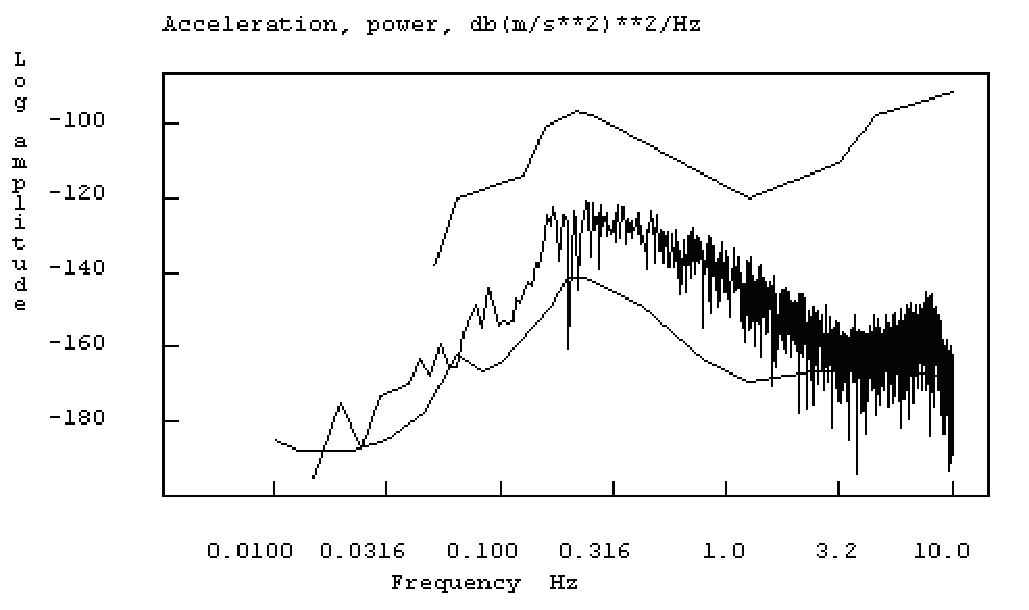
\includegraphics[width=0.9\linewidth]{fig/fig23}}
\caption{Example of a noise spectrum.}
\label{fig:noise-spec}
\end{figure}


\textbf{Problems:}
\index{Problem, MULPLT spectra}There is currently no check if a displacement seismogram has been calculated when calculating the spectral parameters. If spectral analysis is done outside EEV (output in \index{MULPLT.OUT}MULPLT.OUT) or with EEV when there is no origin time and/or epicentral distance, the output results are wrong for moment etc. Before calculating moment etc, the S-file MUST HAVE BEEN UPDATED SINCE BOTH THE DISTANCE AND ORIGIN TIMES ARE USED. If the spectra get very high amplitude levels when correcting for instrument, this might be caused by correcting for Q. With a Q of 100 and a distance of 10 000 km, this gives a very large correction. The Q-correction can be disabled in the \texttt{MULPLT.DEF} file. If picks are made, but no readings appear in the S-file or readings appear with wrong component, the waveform file component might not have been defined in subroutine componen.for. If poles and zeros are used to remove the response,\index{Problem, rotation} rotation cannot be used at the same time. 

\begin{figure}
\htmlimage{scale=2.0}
\centerline{\includegraphics[width=0.9\linewidth]{fig2/fig4a}}
\caption{Spectral analysis\newline
On top the original trace is seen and on the bottom the 
displacement spectrum (log -log, unit nm-sec and Hz). The level 
and slope has been indicated interactively. Note the noise spectrum 
at the bottom of the figure.}
\label{fig:mulplt-spec}
\end{figure}

\begin{figure}
\htmlimage{scale=2.0}
\centerline{\includegraphics[width=0.9\linewidth]{fig2/fig4b}}
\caption{Three component analysis\newline
On top the Z-channel is shown together with the window used for the 
3 channels Z, N and E shown below. The signals below has been filtered 
between 1 and 5 Hz and the resulting azimuth of arrival is 160 degrees 
and a correlation coefficient of 0.2. The apparent velocity is 9.8 km/sec.}
\label{fig:mulplt-3comp}
\end{figure}

\begin{figure}
\htmlimage{scale=2.0}
\centerline{\includegraphics[width=0.9\linewidth]{fig2/fig4c}}
\caption{Plotting response curves\newline
The figure shows the amplitude and phase response for station SUE, 
component S Z. The response is the one which will be used in analysis 
irrespective of whether it is taken from the file header or the CAL directory.}
\label{fig:mulplt-resp}
\end{figure}

\subsection{Particle motion plots}

Particle motion plots can be made in multi trace mode when three components from one station are selected. The particle motion is plotted below the rescaled trace plot. The particle motion plots are made for the time window shown in the trace plot. The trace plot has all the normal functionality, so it is still possible to zoom and filter. The particle motion plots can be useful when determining phase types. No readings can be made from the trace plots. 

\begin{figure}
\htmlimage{scale=2.0}
\centerline{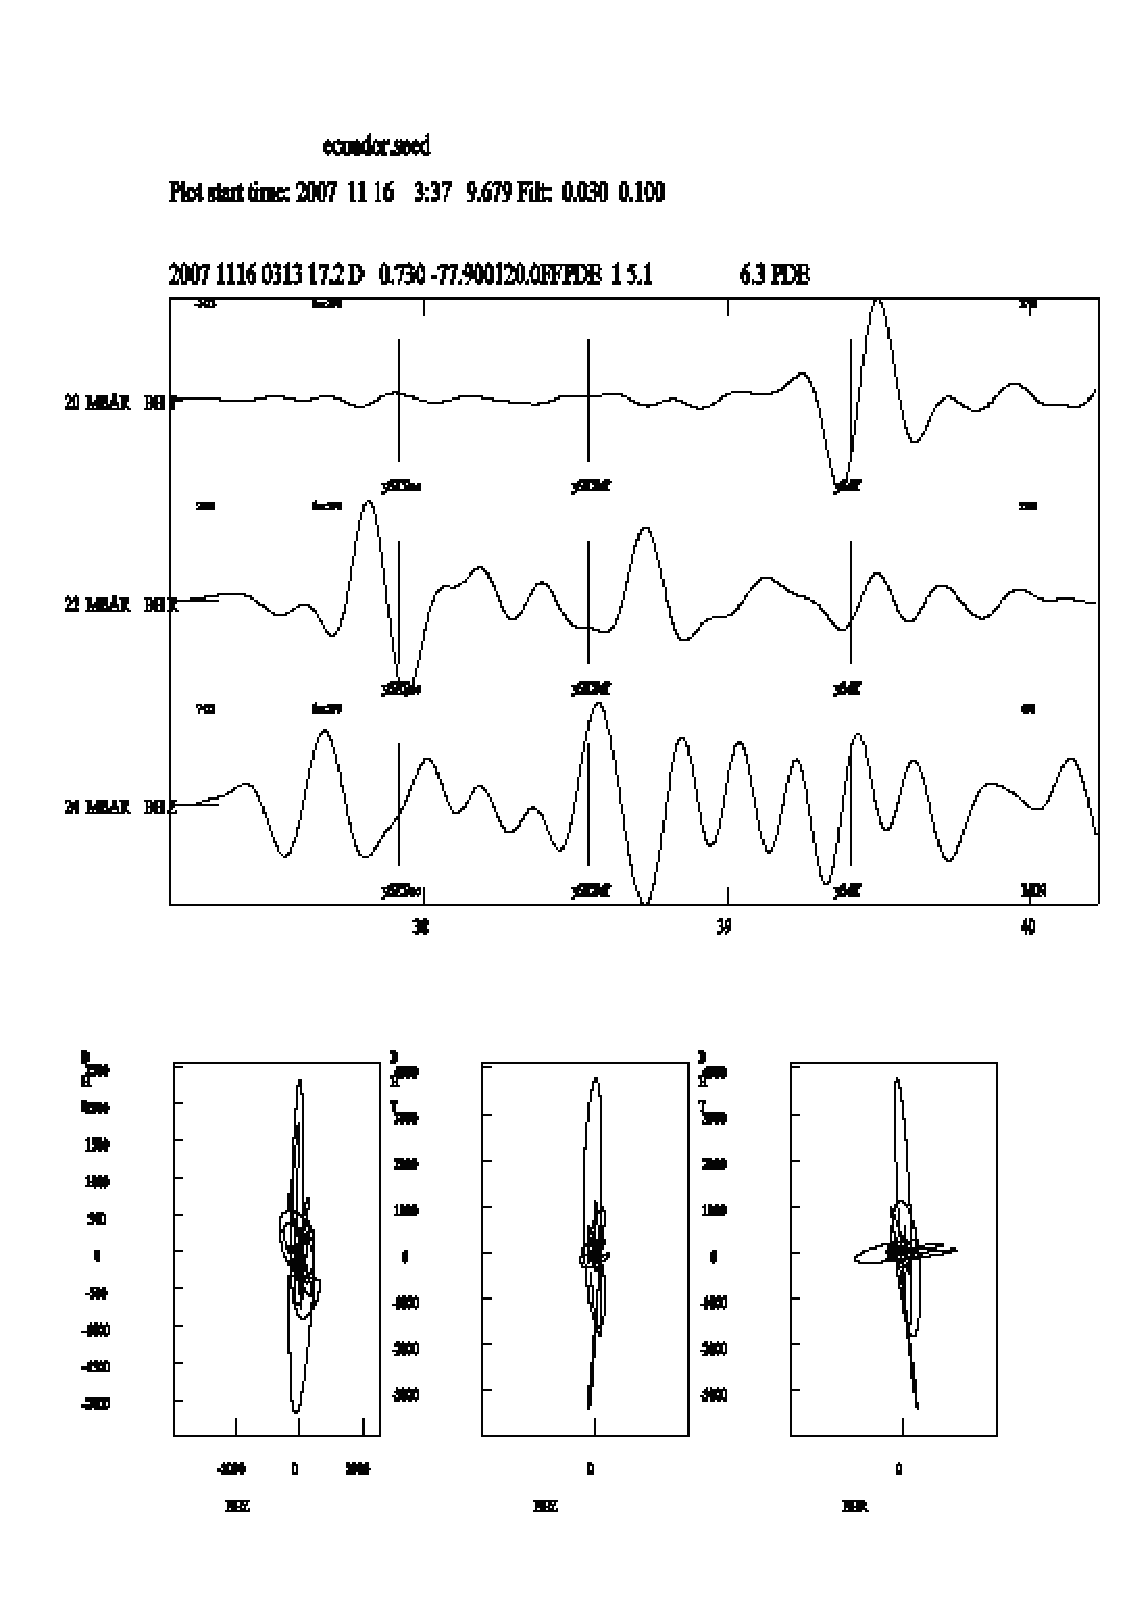
\includegraphics[width=0.9\linewidth]{fig/fig27}}
\caption{Example of particle motion plot.}
%\label{fig:}
\end{figure}

\subsection{The \texttt{MULPLT.DEF} and \texttt{SEISAN.DEF} files}
\index{MULPLT.DEF}\index{SEISAN.DEF}

In the \texttt{MULPLT.DEF} and the \texttt{SEISAN.DEF} files, it is possible to set the various parameters for MULPLT. Nearly all parameters are set in the \texttt{MULPLT.DEF} except geometrical distance parameters, which are set in \texttt{SEISAN.DEF} since these parameters also are used by HYP. MULPLT will operate without DEF-files using \index{Hardwired constants}hardwired defaults. The \texttt{MULPLT.DEF} can be located in the working directory and or in DAT. The if a DEF-file is present in the working directory, it overrides the file in DAT. In \texttt{MULPLT.DEF}, several groups of parameters can be set: The keyboard, default channels to use and analysis parameters (e.g. for spectral analysis). The parameters are identified by keywords, see example file below for explanation.
%\textcolor{red}{jh-change: 
Note that all numbers given in file are real and must be given a '.'

Example file: 

This file is for defaults for MULPLT and called \texttt{MULPLT.DEF}. 
The name must be in upper case on SUN. The following shows the parameters, 
which can be set. The file can contain any number of lines in any order, 
only the lines with recognized keywords and a non blank field under 
Par 1 will be read. 
%\textcolor{red}{pv-change: 
Numbers under Par1 and Par2 must be given as reals.
The comments have no importance. 

%\verbatiminput{include/MULPLT.DEF}
\verbatiminput{../seismo/DAT/DAT/MULPLT.DEF}

All parameters are within column 41 and 60 and each occupying up to 10 characters. 

NOTE: If any of the phase or weight keys are redefined, all previous \index{Defaults}defaults disappear. 

\index{Default channel}\textbf{DEFAULT CHANNEL}: All channels are default if not given. For routine display, it is useful to only select some channels. 

\index{Phase name key}\textbf{PHASE NAME KEY}: The keys associated with given phases. Remember that I, E or a blank MUST be part of the name so it is not possible to chose a name like "P", it must then be " P" (note the blank in front of P). About 10 phase combinations are currently default as seen on the pick display. If a new phase key is selected, you must define all the keys you want to use for phases including all the predefined phases. The combined onset/phase key can be up to 9 characters. 

\index{Phase weight key}\textbf{PHASE WEIGHT KEY}: The defaults are upper 
case 1,2,... to 0 for weights 1,2,... to 0 . Again, choosing just one other 
key, and all must be redefined. The symbol must be in column 41 and the 
weight in column 51. The weight is an integer 0, 1,2,3, 4 or 9. 

\index{Phase mouse key}\textbf{PHASE MOUSE KEY}: The default is blank. Normally no redefinition is needed since the mouse character is defined in SEISAN. The key can be defined as a character or the ASCII code written as a real number. 

\index{Spectral parameters}\textbf{SPECTRAL P-VELOCITY}: P-velocity in km/sec, default 6 km/sec 

\textbf{SPECTRAL S-VELOCITY}: S-velocity in km/sec, default  3.5 km/sec Both above parameters must be set separately, the Vp/Vs in \texttt{STATION0.HYP} is not used to calculate one from the other. The values go into the S-file the first time spectra are calculated. if values are changed later in the \texttt{MULPLT.DEF} file, no change will be made in the S-file, old values remain. 

\textbf{SPECTRAL Q0}:  $Q$ is defined as $q0 * f**qalpha$, default 0 meaning no Q-correction 

\textbf{SPECTRAL QALPHA }: See above, default 1.0, NOTE: Q is only used when doing spectral analysis and has no effect on the displacement seismograms. 

\textbf{SPECTRAL DENSITY}: Density for spectral analysis (g/cm**3), default 3.5 g/cm**3 

\textbf{SPECTRAL KAPPA}: Near surface attenuation, default 0.0 meaning no attenuation. For teleseismic events, this is t*. 

\textbf{SPECTRAL GEO\_DEPTHS}: Depth range where geometrical spreading changes from surface wave to body wave spreading, S-waves only. Default 50 and 100 km. This is only used if distance is larger than HERKIJ\_DISTANCE. THIS PARAMETER IS NOT SET IN \texttt{MULPLT.DEF}, BUT IN \texttt{SEISAN.DEF}, MENTIONED HERE SINCE IT IS IMPORTANT FOR SPECTRA. 

\textbf{HERKIJ\_DISTANCE}: \index{Herkij\_distance}Epicentral distance at which geometrical spreading changes from body wave spreading to surface wave spreading, S-waves only. Default 100 km.  THIS PARAMETER IS NOT SET IN \texttt{MULPLT.DEF}, BUT IN \texttt{SEISAN.DEF}, MENTIONED HERE SINCE IMPORTANT FOR SPECTRA 

\textbf{3COMPVELOCITY}: Velocity used (km/sec) in 3 component azimuth analysis. Default is 5 km/sec. 

\textbf{CHANNEL SORTING}: If set to 1.0, channels and filenames are sorted alphabetically, if 0.0, no sorting. Default = blank is sorting. 

\textbf{NCHAN PER SCREEN}: The number of channels to be displayed per screen. 
Default = blank is 99 channels. 
%\textcolor{red}{pv-change: 
It may conflict with \textbf{DEFAULT CHANNEL}.

\textbf{NSORT\_DISTANCE}: If blank or zero, channels are plotted in 
the order as they appear in the waveform file 
%\textcolor{red}{jh-change:
or in alphabetical order if flag CHANNEL SORTING is set. 
If set to 1.0, the channels are plotted in 
%\textcolor{red}{jh-change: 
distance order if a distance is given in S-file. 
If not plotted from EEV, 1.0 will indicate sorting in 
waveform file header time order. Default 0.

\textbf{X\_SCREEN\_SIZE}: Size of initial X-window in \% of total screen. Default 90 \%. 

\index{Resolution}\textbf{RESOLUTIONX and RESOLUTIONHC is the number of points plotted on the screen or laser printer respectively. If e.g. 1000 points are plotted, this means that the remaining points are skipped although some primitive smoothing is done. Choosing too few points can lead to funny looking seismograms with aliasing effects and using all points will slow down the plotting. Resolutionx is for the screen and resolutionhc for the hardcopy. NOTE}: If using MULPLT mode where both screen and hardcopy is used, it is the hardcopy resolution, which is used for both. Default 1000 and 3000 respectively. 

\textbf{SPECTRAL F-BAND}: Spectral range (Hz) used for spectral plots. Default values are 0.05 to 20.0 Hz. 

\index{AUTO\_PROCESS}\textbf{AUTO\_PROCESS}: Immediately following registration, MULPLT can run any program specified here. Since the event name has been put into memory, the program can operate on the newly \index{Preprocessing of data}registered S-file. Parameter one has the options: 0: Do not auto process, 2: Ask the user if autoprocess, 3: Autoprocess without asking the user. Parameter 2 gives the name of the process to run. The name is limited to 10 characters. Default, no auto processing. 

\index{AUTO\_LOCATE}\textbf{AUTO\_LOCATE}: Immediately following registration, MULPLT can locate the newly registered event and put the location into the database. Parameter one has the options: 0: Do not locate, 1: Ask the user if locate, 2: Locate without asking the user. Parameter 2: 0: Do not save in database, 1: Ask if saving in database, 2: Automatically save in database. Default, no auto locate. 

\textbf{SPECTRAL OUTPUT}: If parameter set to 1, two output files are created for each signal spectrum. \texttt{com\_spec.out} is the complex spectrum and \texttt{amp\_spec.out} is the real spectrum. Default 0.0. In addition, the single trace zoom window is saved in signal.out. 

\textbf{FILTER}: Change definition of filters 1 to 7. The settings affect both the shortcut keys and the menu boxes. 

%\textbf{FILTER TYPE}: Choice between two different filter routines 
%that basically do the same. Use 0.0 for routine 'bndpas' (default) 
%and 1.0 for 'recfil'. Bndpas is a recursive Butterworth bandpass 
%filter routine. Recfil is an IIR filter routine (various filter 
%types supported, but in SEISAN only Butterworth is used), which 
%works as low-, high- or band-pass, however, gives problems for 
%bandpass at low frequencies. Low- and high-pass when using recfil 
%are given by setting either the upper or lower frequency limit to 
%0.0, respectively. 
%\textcolor{red}{jh-change:  
%have remove wa high cut, filters for ms and mb}

\textbf{ML LOW CUT AND POLES and ML HIGH CUT AND POLES}: 
Filter band for Wood Anderson 
%\textcolor{red}{jh-change: 
additional 
filter. Recommanded values are 1.25 Hz to 20 Hz and 4 poles. Note poles for high cut and low cut must be equal, if not lowest value is used. 

\textbf{BANDPASS FILTER}\index{Bandpass filter, default in mulplt}\index{Default filter}: When using all 
defaults from EEV (option PO), a bandpass filter can be set. Default is no filter. The parameters are 
lowcut and highcut for parameter one and two respectively. 4 poles only. 

\textbf{FIX FILTER}\index{Fix filter in mulplt}: When using alldefaults from EEV (option PO), a bandpass filter can be set, see parameter BANDPASS FILTER. The filter can be fixed with paramter FIX FILTER: 1.0 =fix filter, 0=no fix. Fixing means that in all operation the filter will remain.

\textbf{CODA AUTO}: Enable automatic coda determination (YES or NO). Default is NO. If enabled, auto coda is read with c instead of C. 

\textbf{AUTOCODA FILTER }: Filter band for automatic coda: Default 5 to 10 Hz. \index{Coda length}\index{Automatic coda length}AUTOCODA STA : Auto coda short term average: Default 5.0 secs. 

\textbf{AUTOCODA RATIO }: Autocoda ratio. Default 1.5.

\textbf{MULPLT AREA }: Options for plotting stations in a given distance from a midpoint. 0: do not select option (default) 1: midpoint from s-filei epicenter, radius from MULPLT.DEF,  2: midpoint from MULPLT.DEF, radius interactive  3: midpoint and radius from MULPLT.DEF, 4: midpoint from MULPLT.DEF, radius interactive, 5: midpoint and radius interactive 

\textbf{MULPLT LAT LON }: Midpoint 

\textbf{MULPLT RADIUS }: Radius in degrees 

\subsection{Distance trace plot with GMT, TRACE\_PLOT (Unix only)}
\index{TRACE\_PLOT}\index{Trace plotting}
TRACE\_PLOT is a simple program to create a distance trace plot using GMT programs (Generic Mapping Tools, \url{http://gmt.soest.hawaii.edu/}). The axes of the plot are time and distance, and the traces are centered on the respective epicentral distance. The input to the program is a single event in Nordic format (S-file). From the S-file, the program reads the origin time, epicenter location and the names of the associated waveform files. TRACE\_PLOT reads the waveform data and writes the x-y coordinates of the lines in the plot to a file that is then used as input to the GMT program psxy. The TRACE\_PLOT program removes the DC from the data and as an option can apply a band-pass filter. The output of the program is a Postscript file (\texttt{trace\_plot.ps}) and a batch file that can be modified and used to rerun the GMT programs (\texttt{trace\_plot.bat}). The parameters are set in the \texttt{trace\_plot.par} file, which can be located either in the DAT or in the working directory. An example is seen in Figure 
\ref{fig:mulplt-3comp}
. 

The parameters in \texttt{trace\_plot.par} are: 

FILTER: The pass-band filter limits can be specified through the FILTER parameter.\newline
DISTANCE: The distance range (y-axis) for the plot.\newline
TIME: The time range in seconds (x-axis).\newline
AMPLITUDE\_SCALE: The amplitudes are scaled for every trace individually, by  [amplitude/(max 
amplitude) * AMPLITUDE\_SCALE]. \newline
STATION\_SFILE\_ONLY: This variable can be set to 1.0 to only plot 
traces that are listed in the S-file, the default is 0., which plots 
all traces without checking if they are present in the S-file. \newline
TIME\_ORIGIN: In the current version, the origin of the time axis 
corresponds to the origin time of the event. \newline
COMPONENT: This can be used to select components for plotting, in case no component is defined, TRACE\_PLOT will show all vertical component traces. 

Example of \texttt{trace\_plot.par}: 

\verbatiminput{include/trace_plot.par}

